\documentclass[11pt,a4paper]{article}

% ------------------------------------------------------------
% Packages
% ------------------------------------------------------------
\usepackage[utf8]{inputenc}
\usepackage[T1]{fontenc}
\usepackage{lmodern}
\usepackage[a4paper,left=2.5cm,right=2.5cm,top=1.2cm,bottom=2.5cm,includehead,headheight=2.8cm,headsep=0.5cm,footskip=1cm]{geometry}
\usepackage{graphicx}
\usepackage{amsmath,amssymb}
\usepackage{booktabs}
\usepackage{xcolor}
\usepackage{fancyhdr}
\usepackage{titlesec}
\usepackage{listings}
\usepackage{enumitem}
\usepackage[hidelinks]{hyperref}
\usepackage{microtype}
\usepackage{caption}
\usepackage{placeins}
\usepackage{float}
\usepackage[most]{tcolorbox}
\graphicspath{{figures/}}
\captionsetup{font=small,labelfont=bf,skip=8pt}
\definecolor{um6pred}{RGB}{217,74,40}
\tcbset{colback=um6pred!4,colframe=um6pred!65!black,fonttitle=\bfseries,boxrule=.6pt,arc=2mm,left=3mm,right=3mm,breakable}
\setlength{\parskip}{5pt}
\setlength{\parindent}{0pt}
\raggedbottom
\setlength{\textfloatsep}{14pt plus 2pt minus 2pt}
\setlength{\intextsep}{14pt plus 2pt minus 2pt}
\renewcommand{\topfraction}{0.9}
\renewcommand{\bottomfraction}{0.8}
\renewcommand{\textfraction}{0.1}
\renewcommand{\floatpagefraction}{0.7}

% ------------------------------------------------------------
% Colors and code listings
% ------------------------------------------------------------

\definecolor{codebg}{RGB}{242,241,236}

\lstset{
  basicstyle=\ttfamily\small,
  backgroundcolor=\color{codebg},
  frame=single,
  breaklines=true,
  numbers=left,
  numberstyle=\tiny,
  keywordstyle=\color{blue},
  commentstyle=\itshape\color{gray},
  stringstyle=\color{orange!80!black}
}

% ------------------------------------------------------------
% Report information (edit here)
% ------------------------------------------------------------
\newcommand{\ReportTitle}{Symbolic Control Project}
\newcommand{\CourseName}{Computation Theory}
\newcommand{\Professor}{Adnane Saoud}
\newcommand{\Session}{Fall 2026}
\newcommand{\Program}{Computer Engineering} % change or remove if needed
\newcommand{\RepoLink}{\texttt{https://github.com/...}}

% Logos: place UM6P_logo.png and CC_logo.png in the figures folder.
% If they are missing, text placeholders are used so the file still compiles.
\newcommand{\UMlogo}[1]{\IfFileExists{figures/UM6P_logo.png}{
\includegraphics[height=#1]{figures/UM6P_logo.png}}{\textbf{\color{um6pred}UM6P}}}
\newcommand{\CClogo}[1]{\IfFileExists{figures/CC_logo.png}{
\includegraphics[height=#1]{figures/CC_logo.png}}{\textbf{College of Computing}}}

% ------------------------------------------------------------
% Header / footer
% ------------------------------------------------------------
\pagestyle{fancy}
\fancyhf{}
\lhead{\vtop{\hbox{\UMlogo{2.5cm}}}}
\rhead{\vtop{\hbox{\CClogo{2.1cm}}}}
\renewcommand{\headrulewidth}{0.4pt}
\lfoot{Symbolic Control Project}
\cfoot{Page \thepage}
\rfoot{Prof.\ \Professor}
\renewcommand{\footrulewidth}{0pt}

% Part and section style
\titleformat{\part}[display]{\centering\Huge\bfseries\color{um6pred}}{Part \thepart}{10pt}{}
\titlespacing*{\part}{0pt}{12pt}{24pt}
\titleformat{\section}{\Large\bfseries\color{um6pred}}{\thesection}{1em}{}
\titleformat{\subsection}{\large\bfseries}{\thesubsection}{1em}{}
\titleformat{\subsubsection}{\normalsize\bfseries}{\thesubsubsection}{1em}{}
\titleformat{\paragraph}[block]{\normalsize\bfseries}{}{0pt}{}
\titlespacing*{\paragraph}{0pt}{10pt}{4pt}

\setlist[itemize]{itemsep=2pt}
\setlist[enumerate]{itemsep=2pt}

% ============================================================
\begin{document}

% ------------------------------------------------------------
% Title page
% ------------------------------------------------------------
\begin{titlepage}
  \thispagestyle{empty}
  \vspace*{-3.2cm}
  \noindent
  \vtop{\hbox{\UMlogo{3.8cm}}}\hfill\vtop{\hbox{\CClogo{3.2cm}}}

  \vspace{2.5cm}
  \begin{center}
    {\LARGE\bfseries \ReportTitle\par}
    \vspace{1cm}
    {\Large\bfseries \CourseName\ Course\par}
    \vspace{0.2cm}
    {\large UM6P College of Computing\par}
    \vspace{0.8cm}
    \textbf{Professor:} \Professor \quad
    \textbf{Program:} \Program\\[2pt]
    \textbf{Session:} \Session
  \end{center}

  \vspace{1.2cm}
  \hrule
  \vspace{0.6cm}
  \begin{center}
    {\large\bfseries Team Information}\\[8pt]
    \renewcommand{\arraystretch}{1.15}
    \begin{tabular}{|l|l|}
      \hline
      \textbf{Member 1} & Omar Tsouli \\ \hline
      \textbf{Member 2} & Aymane Raiss \\ \hline
      \textbf{Member 3} & Amine Chrif \\ \hline
      \textbf{Member 4} & Rayane Khaldi \\ \hline
      \textbf{Member 5} & Younes Lougnidi \\ \hline
      \textbf{Repository Link} & \RepoLink \\ \hline
    \end{tabular}
  \end{center}
  \vspace{0.3cm}
  \hrule
\end{titlepage}

% ------------------------------------------------------------
% Table of contents
% ------------------------------------------------------------
\pagenumbering{arabic}
\setcounter{page}{1}
\thispagestyle{fancy}
\tableofcontents
\clearpage

% ============================================================
\part{Mobile Robot Symbolic Control}
\label{part:mobile-robot}

\section{Introduction}
% ============================================================

\subsection{Context and Objective}

In this first part of the project, we apply symbolic control to a \textbf{mobile robot navigation problem}: a
unicycle-type robot, subject to bounded disturbances and to state and input constraints, must
satisfy a temporal specification over several regions of its workspace. Our work follows the
approach presented in the reference article by Girard, Meyer and Saoud,
\emph{Approches symboliques pour le contr\^ole des syst\`emes non lin\'eaires}
(Techniques de l'Ing\'enieur, 2024), and the project statement provided in class.

\subsection{Problem Overview}

The robot evolves in the plane. Its state is its position and heading
$x(t)=(x_1(t),x_2(t),x_3(t))$, and it is controlled through its linear and angular velocities
$u(t)=(u_1(t),u_2(t))$. In discrete time, and under a bounded disturbance $w(t)$, its dynamics take the
generic form
\begin{equation}
  x(t+1) = f\big(x(t),u(t),w(t)\big),\qquad x(t)\in X,\; u(t)\in U,\; w(t)\in W,
\end{equation}
where $X$, $U$ and $W$ are compact sets encoding the state constraints, the input
constraints and the disturbance bounds, respectively. The model and discretization choices
are detailed in Section~\ref{sec:abstraction}.

We consider three control specifications over the workspace, of increasing complexity. The
regions $R_1,\dots,R_4$ are disjoint subsets of the state space.
\begin{enumerate}
  \item \textbf{Reachability (going from one state to another).} Starting from an initial
  region, the robot must reach a given target region in finite time.
  \item \textbf{Safety (avoiding an obstacle).} The robot must never enter the obstacle
  region, at any time.
  \item \textbf{Temporal specification.} This specification combines reachability and safety
  over the four regions:
  \begin{quote}
    \emph{``Go to $R_1$ or to $R_2$, but only to one of them, then to $R_3$,
    while avoiding $R_4$ all the way.''}
  \end{quote}
\end{enumerate}
The first two are elementary specifications, for which a static state-feedback controller is
sufficient. The third goes beyond classical stability objectives: it is a co-safe LTL property
that can be captured by a finite-state automaton, and its controller requires memory.

\subsection{Work Plan}

To structure the work, we divided the project into four consecutive steps. Each step builds
on the previous one, which lets us validate the theory before implementing it and validate
the implementation before using it to synthesize a controller.

\begin{enumerate}
  \item \textbf{Abstraction and reachability: theory.} We identified the parts of the
  reference article that formalize symbolic abstraction and reachability analysis, namely
  Section~1.1 (abstraction methodology) and Sections~3.1 and~3.2 (model, specification,
  abstraction and controller synthesis for the mobile robot). The goal of this step is to
  understand and document how the state and input spaces are discretized and how the
  symbolic transition function is obtained by over-approximating reachable sets.

  \item \textbf{Abstraction and reachability: implementation.} We will implement the methods
  described in the first step, namely the partition of the state space, the quantization of
  the inputs, and the computation of the transition function through reachability analysis.
  This implementation is the foundation on which all subsequent steps are built.

  \item \textbf{Controller synthesis: theory and implementation.} We will study the synthesis
  methods presented in Section~2 of the article, in particular the treatment of
  automaton-based specifications through a product between the symbolic model and the
  specification automaton. We will then implement the synthesis algorithm on top of the
  abstraction developed in step~2.

  \item \textbf{Concretization and real-time control.} Finally, we will bring the work together
  by going from the symbolic controller to a controller applicable to the real robot
  dynamics (Section~1.2 of the article), and validate it through numerical simulations
  (Section~3.3).
\end{enumerate}

\subsection{Report Organization}

This part of the report follows these four steps. Section~\ref{sec:abstraction} presents
the model, the specification, and the abstraction and reachability analysis (steps 1 and 2),
Section~\ref{sec:synthesis} covers controller synthesis (step 3), and
Section~\ref{sec:concretization} covers the concretization of the controller and the
simulation results (step 4). At this stage, only the theory of abstraction
has been documented; implementation and subsequent stages remain to be completed.

% ============================================================
\section{Symbolic Abstraction and Reachability Analysis}
\label{sec:abstraction}
% ============================================================


\subsection{Theory}

\begin{tcolorbox}[title={First meeting --- 7 October 2026}]
During our first meeting on 7 October 2026, we discussed the abstraction
method step by step. We first worked through
Section~1.1 of the reference article, then connected its definitions to the
mobile robot in Sections~3.1 and~3.2. Our objective was to understand what
each symbolic state represents, how uncertainty produces several possible
successors, and how reachable sets can be enclosed safely.
This section records our understanding at the end of that meeting.
\end{tcolorbox}

\FloatBarrier
\subsubsection{From a continuous state space to a finite model}
We started from the discrete-time system
\[
 x(t+1)=f(x(t),u(t),w(t)),\qquad x(t)\in X,\quad u(t)\in U,\quad w(t)\in W,
\]
where $X$, $U$ and $W$ are compact constraint sets. Here ``continuous''
refers to the possible values of the state, whereas time is discrete.
We understood symbolic abstraction as replacing this infinite collection
of states and commands by a finite description:
\[
 \xi(t+1)\in g(\xi(t),\sigma(t)),\qquad \xi(t)\in X_s,\quad \sigma(t)\in U_s.
\]
The transition map $g$ is set-valued. Even after choosing a command, we
do not know the exact point within the current cell or the disturbance.
Several successors must therefore remain possible.

\begin{figure}[H]
 \centering
 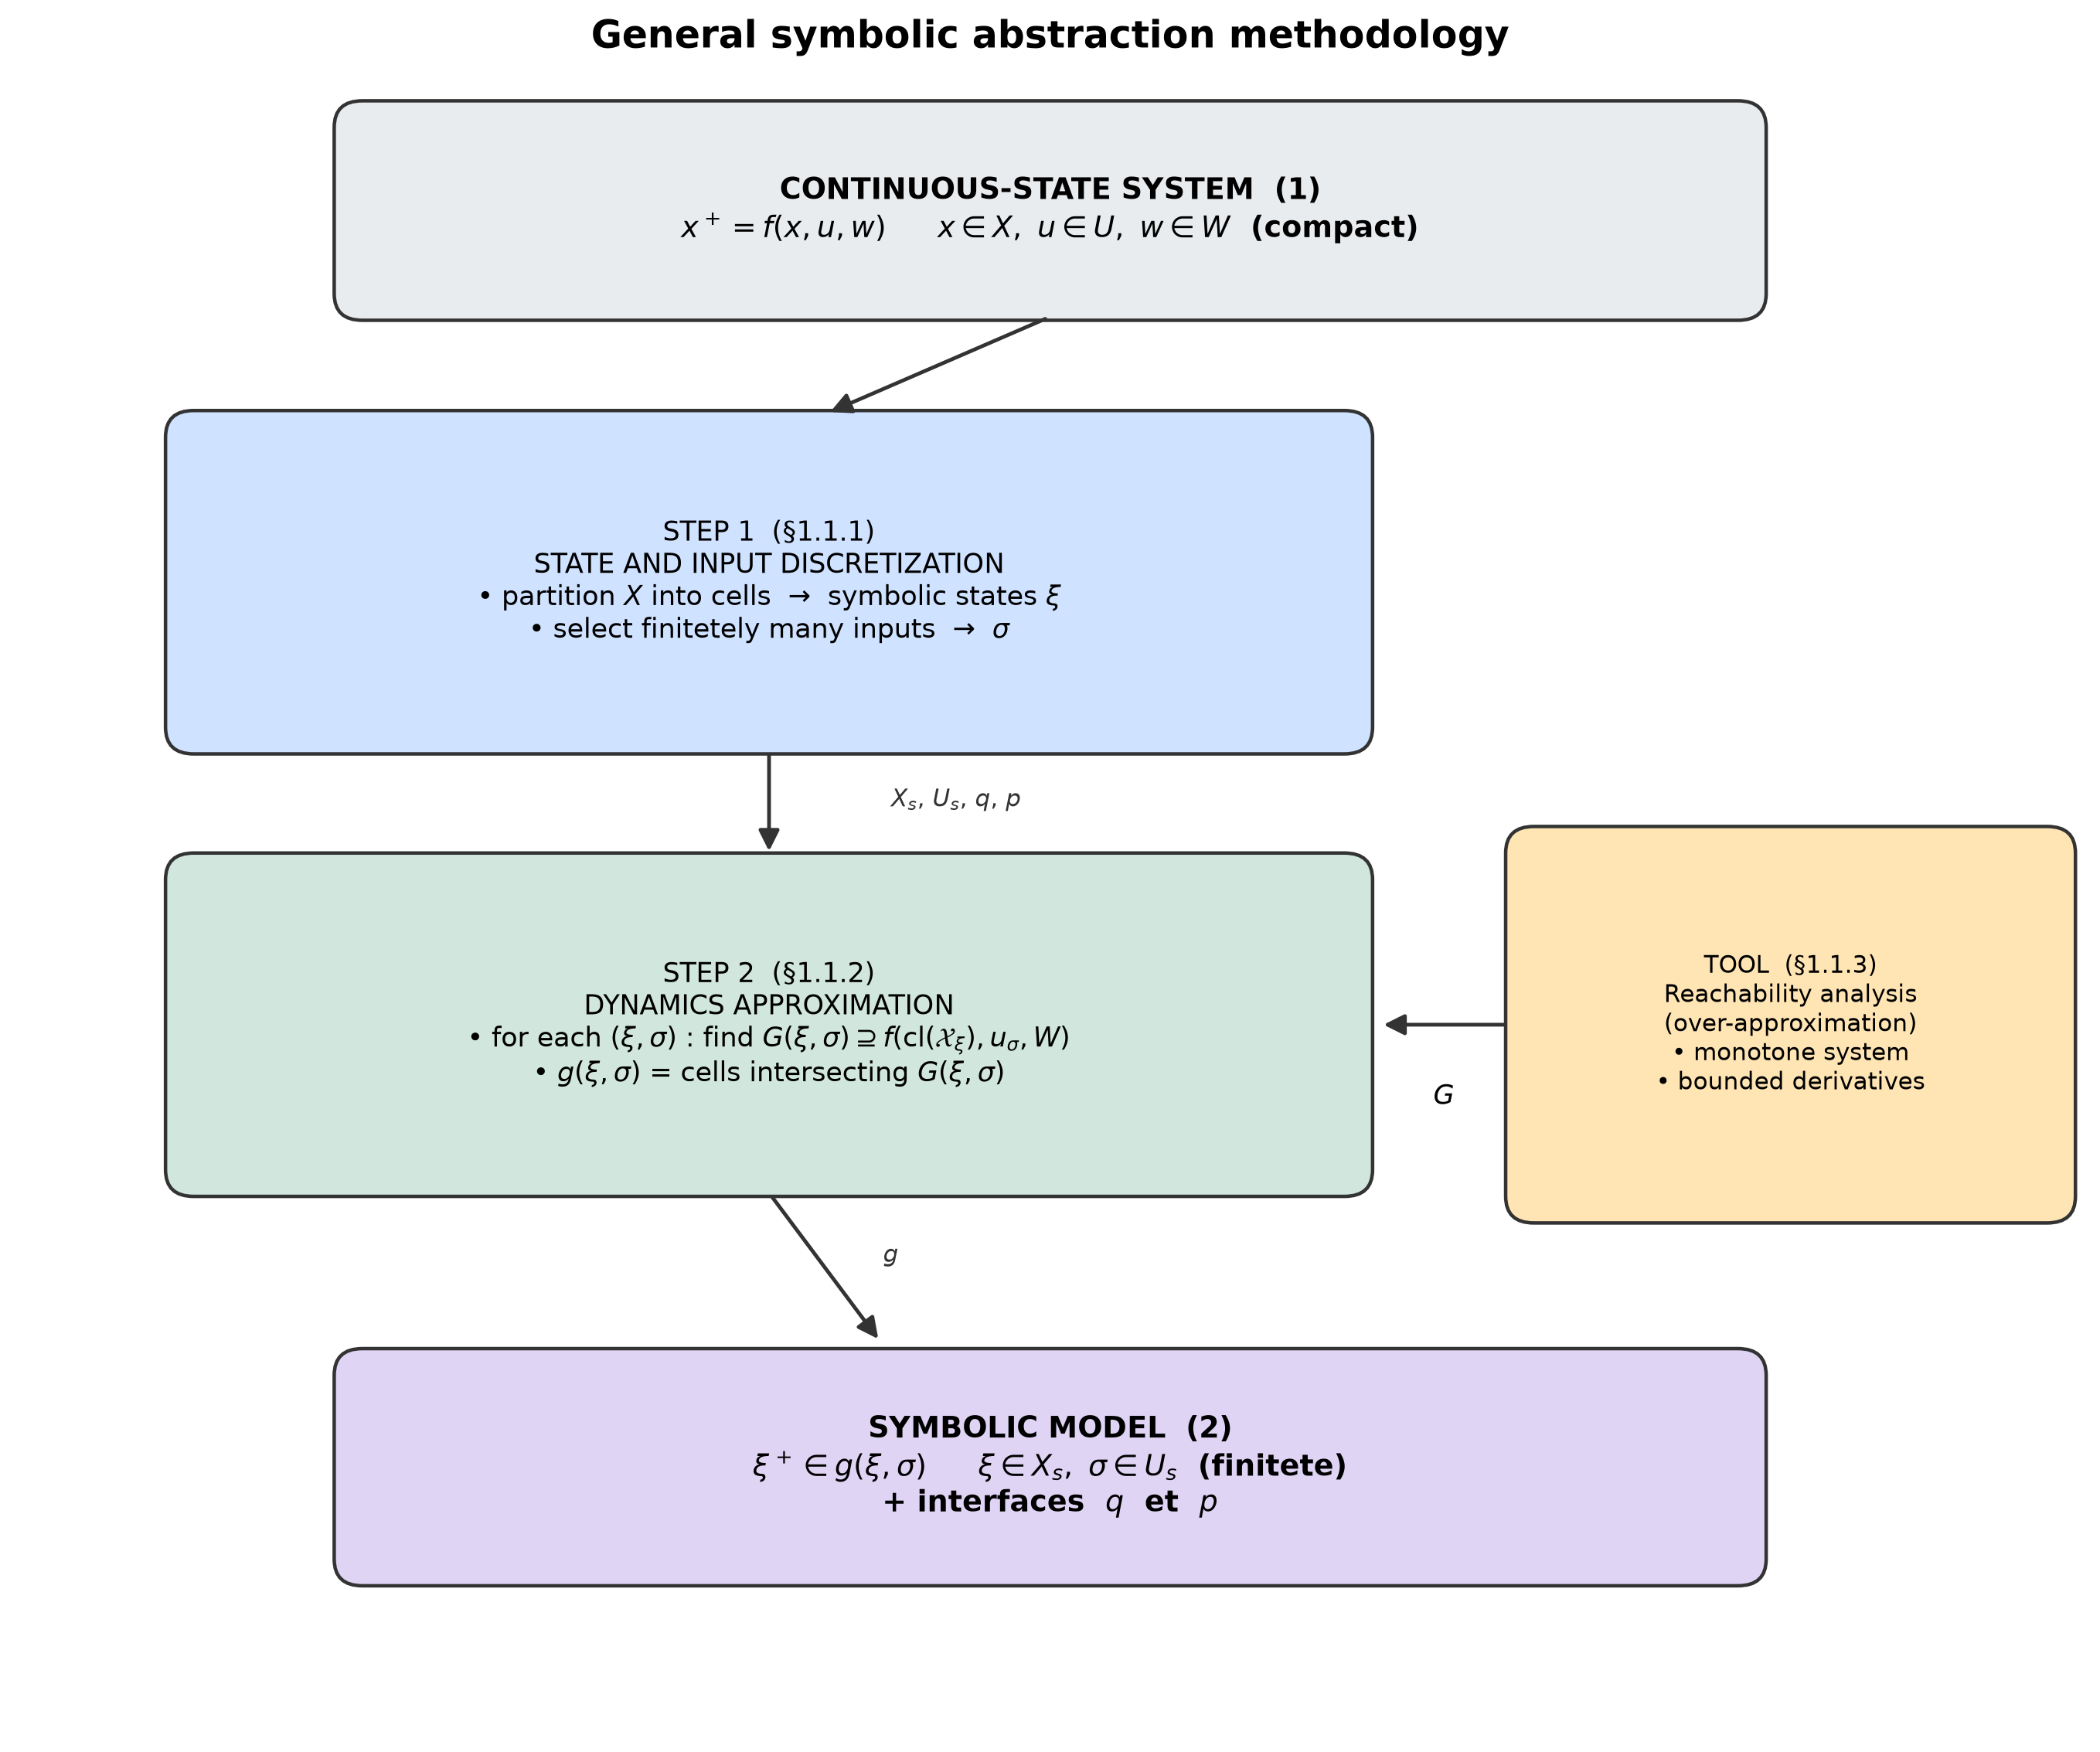
\includegraphics[width=.88\linewidth,height=.58\textheight,keepaspectratio]{abstraction_workflow.png}
 \caption{The two stages we studied: discretizing states and inputs, then
 enclosing their possible next states.}
\end{figure}

\FloatBarrier
\subsubsection{Partitioning states and selecting commands}
We partition $X$ into $m$ cells $\mathcal X_1,\ldots,\mathcal X_m$ and
associate one symbolic state $\xi_i$ with each cell. An additional state
$\xi_0$ represents $\mathcal X_0=\mathbb R^n\setminus X$:
\[
 X_s=\{\xi_0,\xi_1,\ldots,\xi_m\}.
\]
Cell boundaries need a consistent assignment so that each point in $X$
belongs to exactly one cell. The abstraction interface is
\[
 q(x(t))=\xi_i\quad\text{when }x(t)\in\mathcal X_i.
\]
For the inputs, we select finitely many admissible values
$u_1,\ldots,u_l\in U$. We then define
\[
 U_s=\{\sigma_1,\ldots,\sigma_l\},\qquad p(\sigma_j)=u_j.
\]
The distinction that helped us most is that a symbolic state represents
\emph{an entire set of points}, while a symbolic command represents
\emph{one selected input value}. The map $q$ reads the robot state at
the symbolic level; $p$ translates a symbolic command into a real input.

\begin{figure}[H]
 \centering
 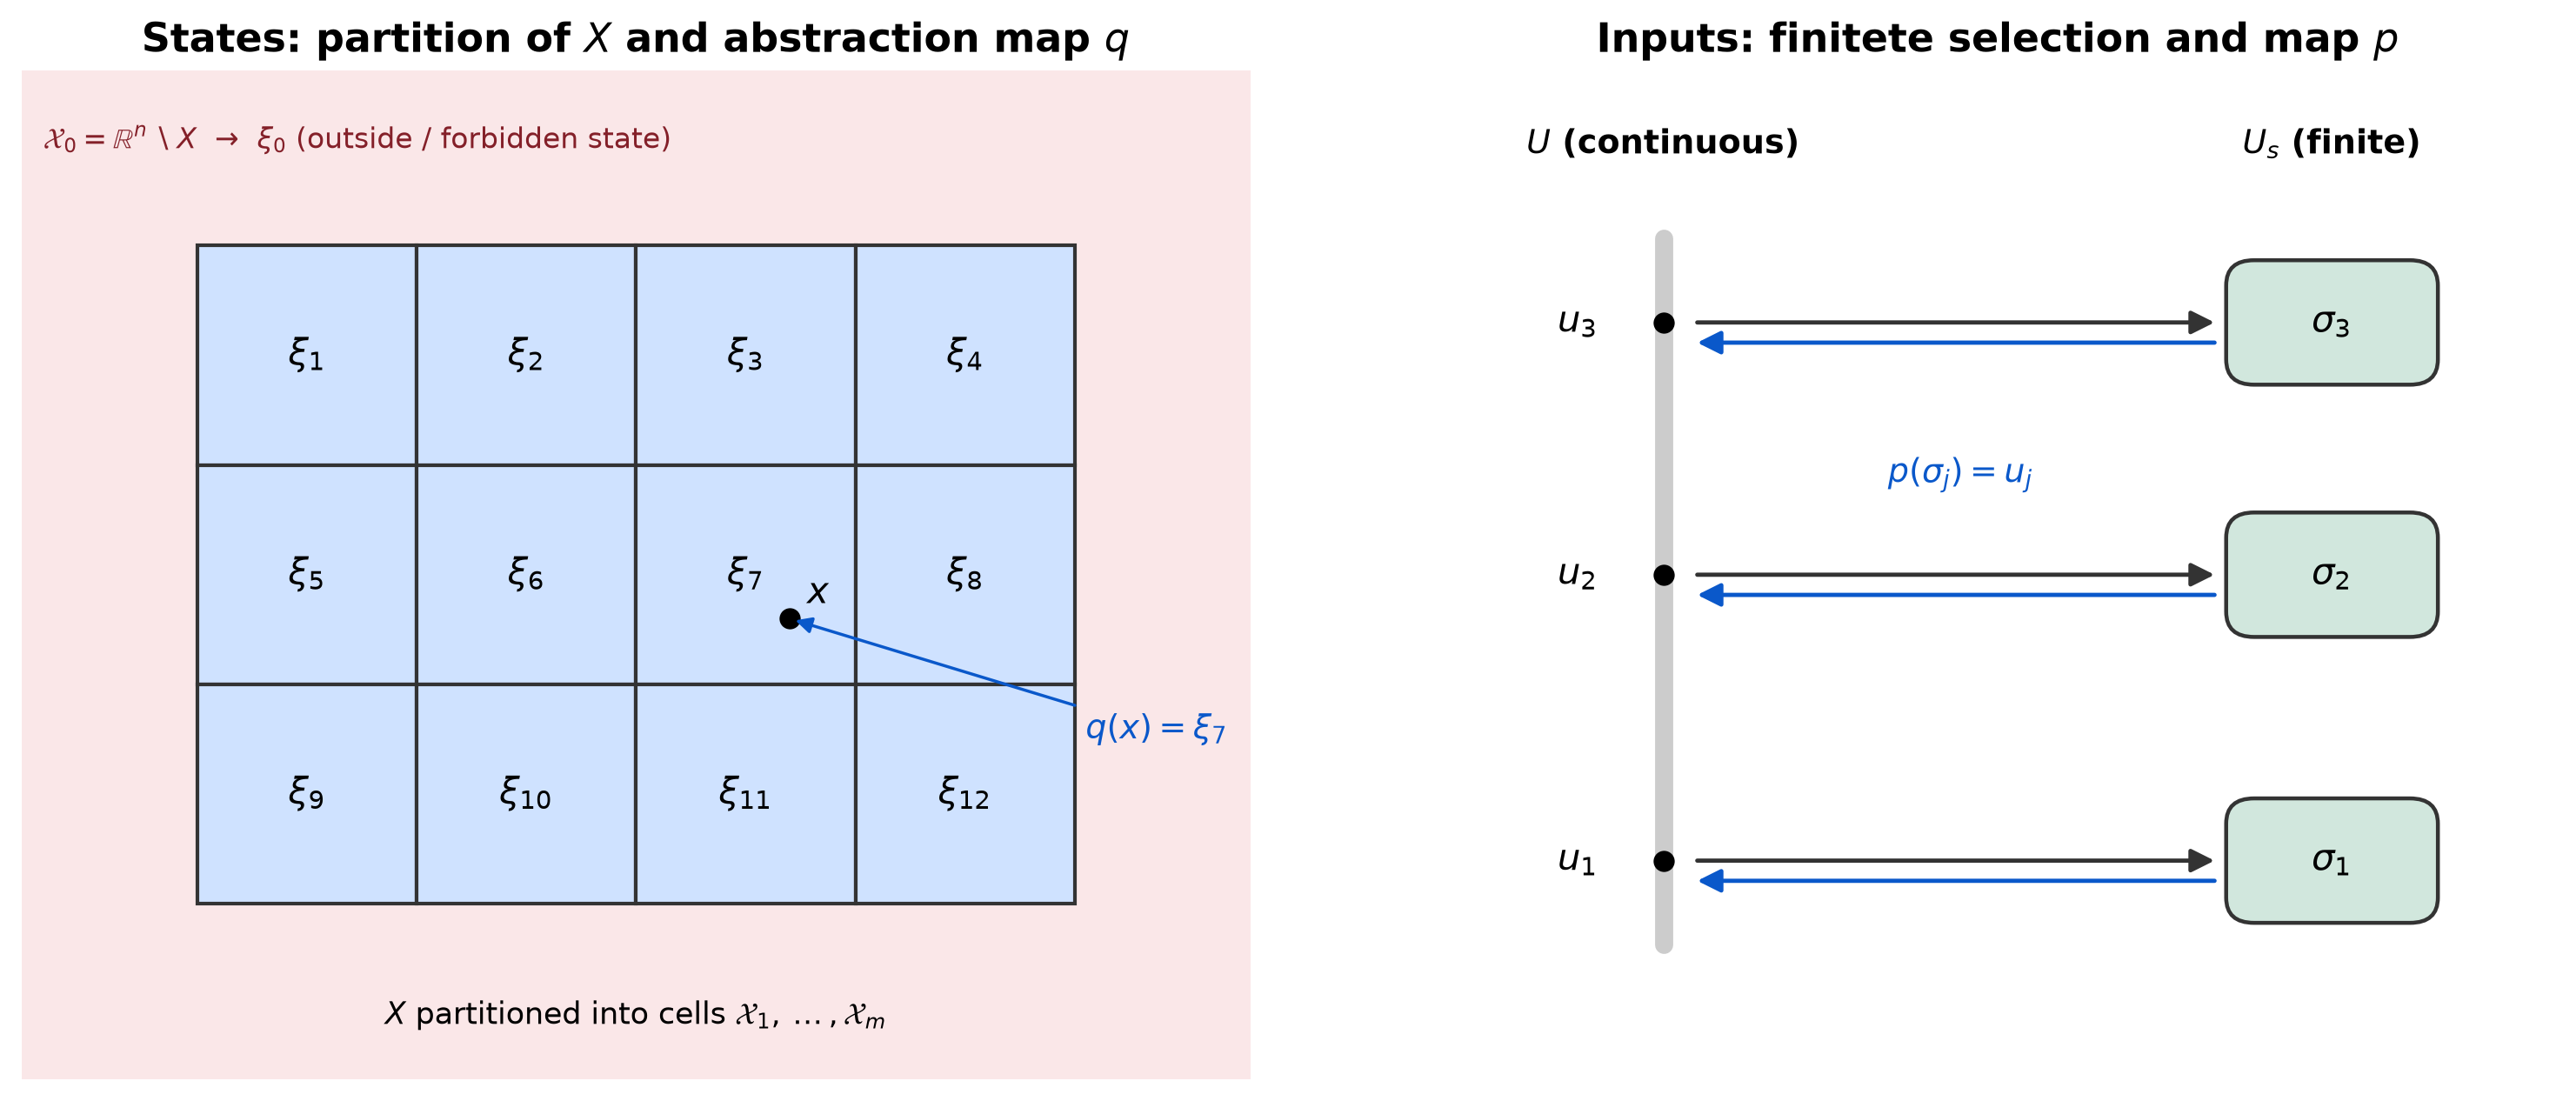
\includegraphics[width=\linewidth,height=.43\textheight,keepaspectratio]{state_input_discretization.png}
 \caption{State cells, the outside state, and the interfaces $q$ and $p$.
 The small grid illustrates the definitions; it is not the robot's full grid.}
\end{figure}

\FloatBarrier
\subsubsection{Defining transitions through over-approximation}
For a fixed cell and command, the one-step reachable set is
\[
 \mathcal R(\xi,\sigma)=
 \{f(x(t),u_\sigma,w(t)):x(t)\in\operatorname{cl}(\mathcal X_\xi),\ w(t)\in W\}.
\]
The closure includes the cell's boundary when computing a safe enclosure.
Computing this set exactly is often difficult for nonlinear dynamics, so
we construct a simpler set $G(\xi,\sigma)$ satisfying
\begin{equation}
 \mathcal R(\xi,\sigma)\subseteq G(\xi,\sigma).
 \label{eq:enclosure}
\end{equation}
We retain every cell touched by that enclosure:
\begin{equation}
 g(\xi,\sigma)=\{\xi'\in X_s:
 \mathcal X_{\xi'}\cap G(\xi,\sigma)\ne\varnothing\}.
 \label{eq:successors}
\end{equation}
In particular, if $G$ intersects the complement of $X$, the outside state
is a possible successor. This makes a possible violation of the state
constraint visible in the finite model.

\begin{figure}[H]
 \centering
 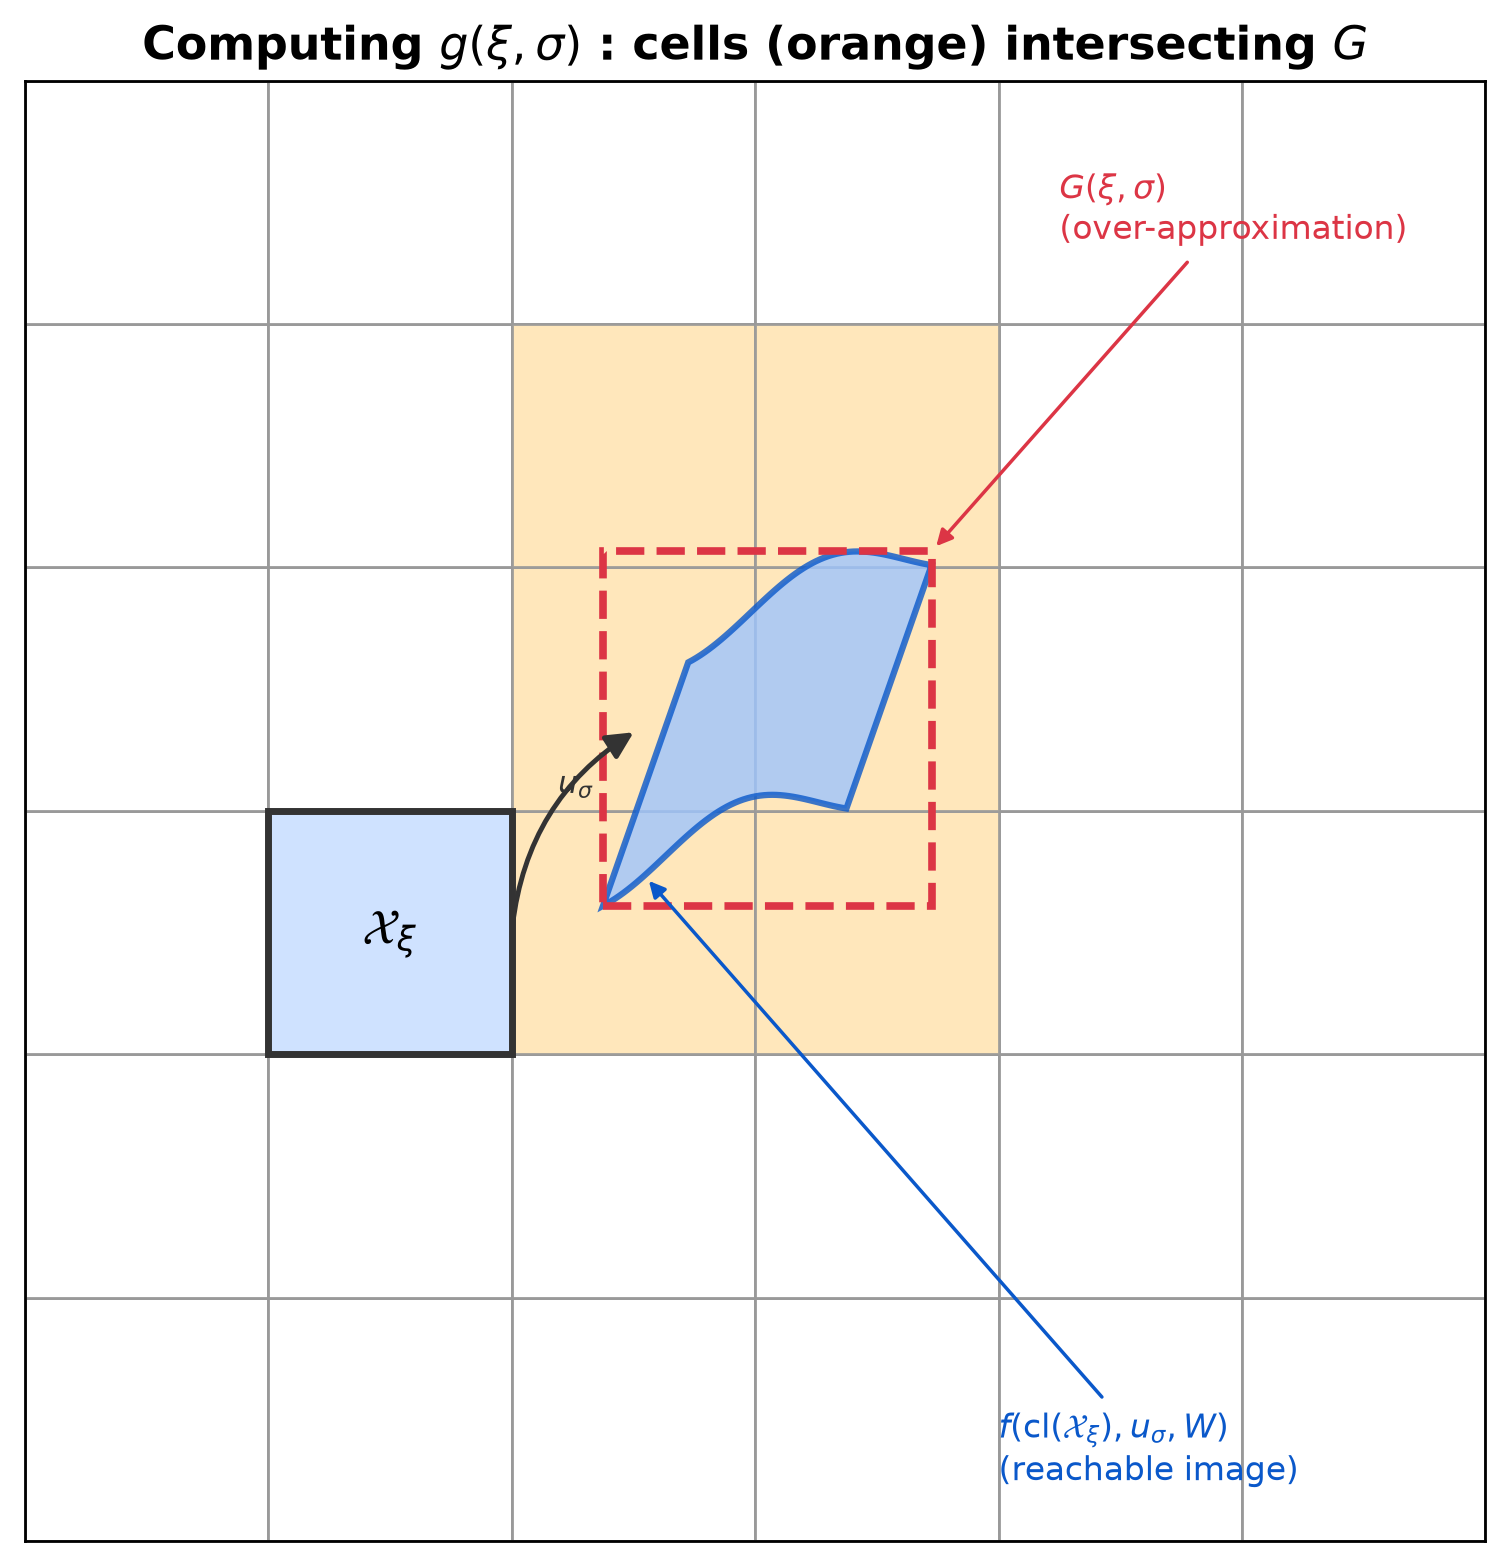
\includegraphics[width=.68\linewidth,height=.43\textheight,keepaspectratio]{transition_overapproximation.png}
 \caption{The source cell is blue, the
 reachable image is enclosed by the dashed box $G$, and the orange cells
 become symbolic successors. This is a schematic example, not a robot simulation.}
\end{figure}

\begin{tcolorbox}[title={What we understood about uncertainty}]
We choose the command, but we cannot choose which successor occurs.
The abstraction must cover every admissible disturbance and every point
in the source cell. A larger enclosure is safe but may introduce
transitions that the physical system cannot actually realize.
\end{tcolorbox}

\FloatBarrier
\subsubsection{Two ways to enclose a reachable set}
We compared two interval-based methods. All inequalities below are
componentwise, and $[a,b]$ denotes a multidimensional box.

\paragraph{Monotone dynamics.}
Following Section~1.1.3 of the article, we
first considered a differentiable system for which every entry of the
state and disturbance Jacobians is nonnegative:
\[
 \frac{\partial f_i}{\partial x_j(t)}\ge0
 \qquad\text{and}\qquad
 \frac{\partial f_i}{\partial w_k(t)}\ge0
 \qquad (\text{for all }i,j,k).
\]

This implies the following order-preserving property:
\[
 \begin{aligned}
 &x(t)\le\widetilde x(t),\qquad w(t)\le\widetilde w(t)\\[6pt]
 &\quad\Longrightarrow\quad f(x(t),u_\sigma,w(t))
 \le f(\widetilde x(t),u_\sigma,\widetilde w(t)).
 \end{aligned}
\]
Here vector inequalities compare corresponding coordinates, rather than
vector lengths. For example, $x(t)\le\widetilde x(t)$ means
$x_j(t)\le\widetilde x_j(t)$ for every $j$.

We then take a cell and disturbance set represented by boxes:
\[
 \operatorname{cl}(\mathcal X_\xi)=[\underline x,\overline x],
 \qquad W=[\underline w,\overline w].
\]
The vectors $\underline x$ and $\overline x$ contain the lower and upper
coordinate bounds of the current cell; they are fixed bounds. Thus every admissible pair satisfies
\[
 \underline x\le x(t)\le\overline x,\qquad
 \underline w\le w(t)\le\overline w.
\]
Applying the order-preserving property twice gives
\[
 \begin{aligned}
 f(\underline x,u_\sigma,\underline w)
 &\le x(t+1)=f(x(t),u_\sigma,w(t))\\
 &\le f(\overline x,u_\sigma,\overline w).
 \end{aligned}
\]
Therefore we only need to compute two successors: one from the lower
state and disturbance corners, and one from the upper corners. They
define the enclosure
\[
 G(\xi,\sigma)=
 \big[f(\underline x,u_\sigma,\underline w),
      f(\overline x,u_\sigma,\overline w)\big].
\]
We understood why this is the \emph{smallest enclosing box}: every
reachable state lies between these two vectors, and both corner images
are themselves reachable from the closed cell and disturbance box.

\paragraph{Bounded derivatives.}
If monotonicity is unavailable, we instead bound the absolute values of
the derivatives throughout the relevant domain:
\[
 \left|\frac{\partial f}{\partial x(t)}\right|\le D_x,
 \qquad
 \left|\frac{\partial f}{\partial w(t)}\right|\le D_w.
\]
For the current cell $\operatorname{cl}(\mathcal X_\xi)=[\underline x,\overline x]$
and disturbance box $W=[\underline w,\overline w]$, we compute the centres
and half-widths componentwise, as in the article:
\[
 \begin{aligned}
 x^*(t)&=\frac{\underline x+\overline x}{2}, &
 \delta x&=\frac{\overline x-\underline x}{2},\\[4pt]
 w^*&=\frac{\underline w+\overline w}{2}, &
 \delta w&=\frac{\overline w-\underline w}{2}.
 \end{aligned}
\]
Here $x^*(t)$ is the centre of the cell containing $x(t)$, not the exact
measured state. For a symmetric disturbance box, $w^*=0$.
The centre of the enclosure is obtained by evaluating the dynamics at
these two midpoints, under the selected command:
\[
 \begin{aligned}
 c&=f(x^*(t),u_\sigma,w^*)\\[4pt]
  &=f\!\left(\frac{\underline x+\overline x}{2},u_\sigma,
             \frac{\underline w+\overline w}{2}\right).
 \end{aligned}
\]
The half-width and the resulting enclosure are
\begin{equation}
 \begin{gathered}
 r=D_x\delta x+D_w\delta w,\\[4pt]
 G(\xi,\sigma)=[c-r,c+r].
 \end{gathered}
 \label{eq:bounded-derivatives}
\end{equation}
We interpreted $c$ as the nominal next state (because it is the state
predicted at time $t+1$ when the current state is taken at the cell centre
and the disturbance at its centre, under the selected command $u_\sigma$).
It is the image of the input centres, not necessarily the midpoint of the
exact reachable set. The vector $r$ covers the variation inside the cell
and the disturbance box. This method requires one evaluation of $f$ at
these centres once valid derivative bounds are available.

\begin{figure}[H]
 \centering
 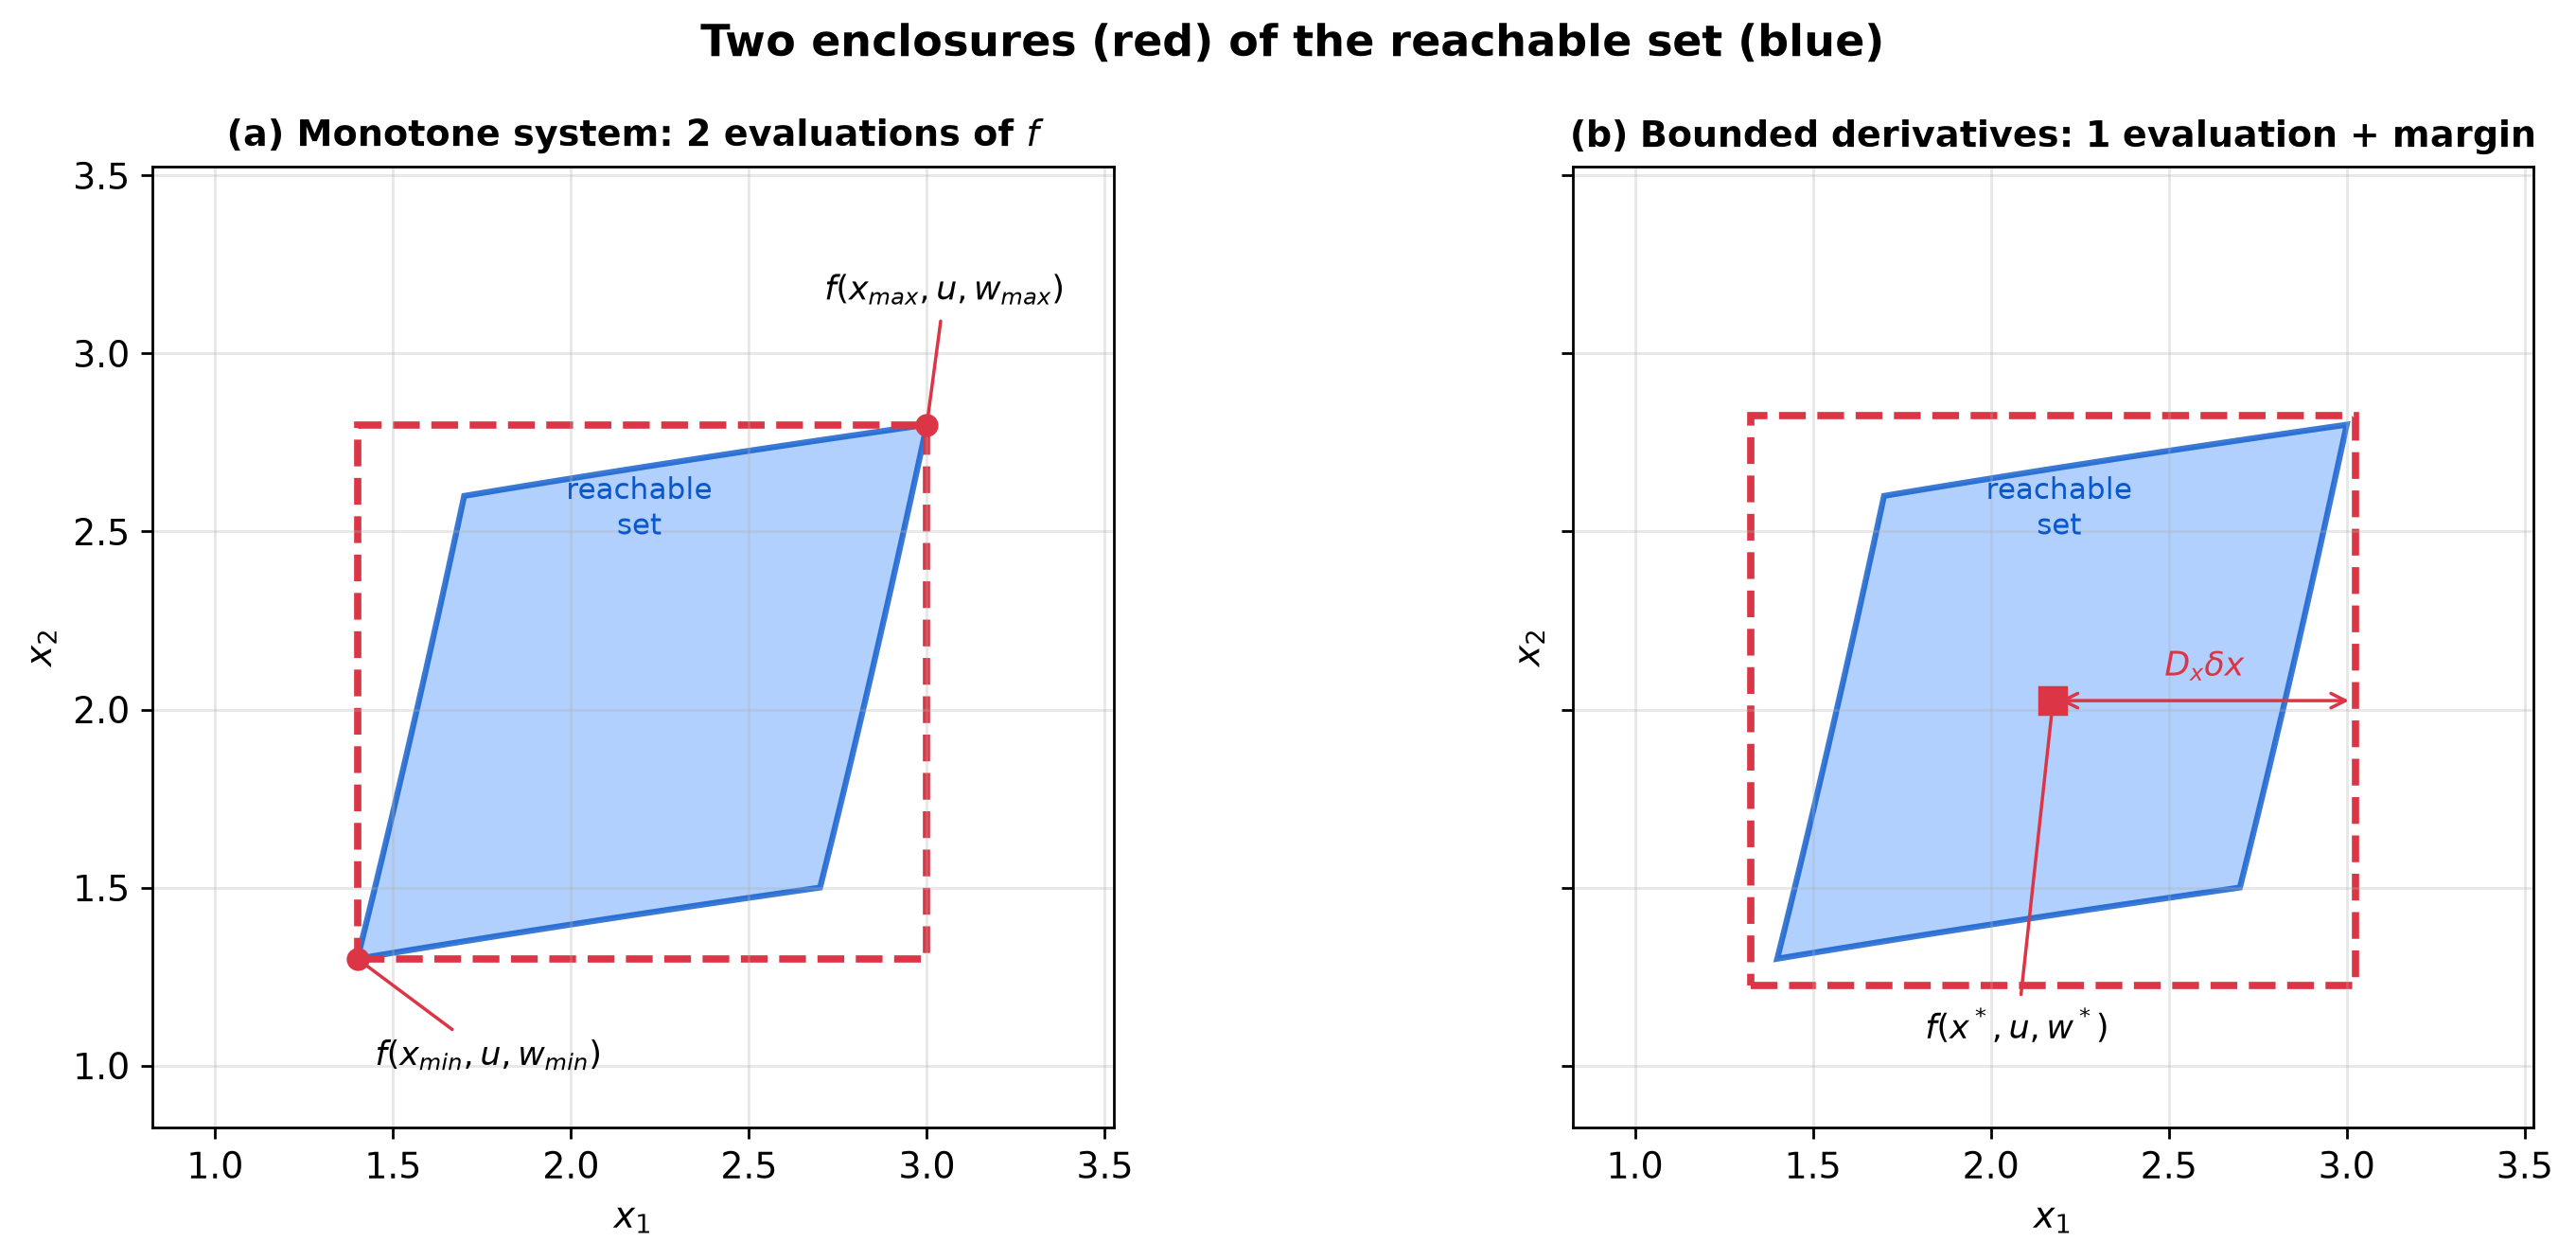
\includegraphics[width=\linewidth,height=.43\textheight,keepaspectratio]{reachability_methods_english.png}
 \caption{Comparison of reachability methods: corner
 bounds for a monotone system (left) and a centre-based enclosure using
 bounded derivatives (right).}
\end{figure}

We also discussed the balance between precision and size. Finer state
partitions provide more detail but increase the number of symbolic states.
Loose enclosures create more possible successors and can make later
controller synthesis conservative. In particular, if every command allows
a self-transition, the abstraction can fail to certify progress toward a
target. This observation guided our understanding of the discretization choices.

\FloatBarrier
\FloatBarrier
\subsubsection{Applying the method to the mobile robot: Section 3.1}
We then connected these definitions to a unicycle robot. Its state is
$x(t)=(x_1(t),x_2(t),x_3(t))$, where the first two coordinates describe position and
$x_3(t)$ is the heading. The commands $u_1(t)$ and $u_2(t)$ are its linear and
angular velocities. We consider the sampled model
\begin{equation}
 \begin{aligned}
 x_1(t+1)&=x_1(t)+\tau(u_1(t)\cos x_3(t)+w_1(t)),\\
 x_2(t+1)&=x_2(t)+\tau(u_1(t)\sin x_3(t)+w_2(t)),\\
 x_3(t+1)&=x_3(t)+\tau(u_2(t)+w_3(t)).
 \end{aligned}
 \label{eq:robot}
\end{equation}
Here $\tau$ is the sampling period and $w(t)$ is a bounded disturbance.
The position moves along the current heading, while the angular command
changes that heading. The sine and cosine terms make this model nonlinear.
The heading equation is written in a local angular coordinate; the course
statement treats heading modulo $2\pi$.

\begin{figure}[H]
 \centering
 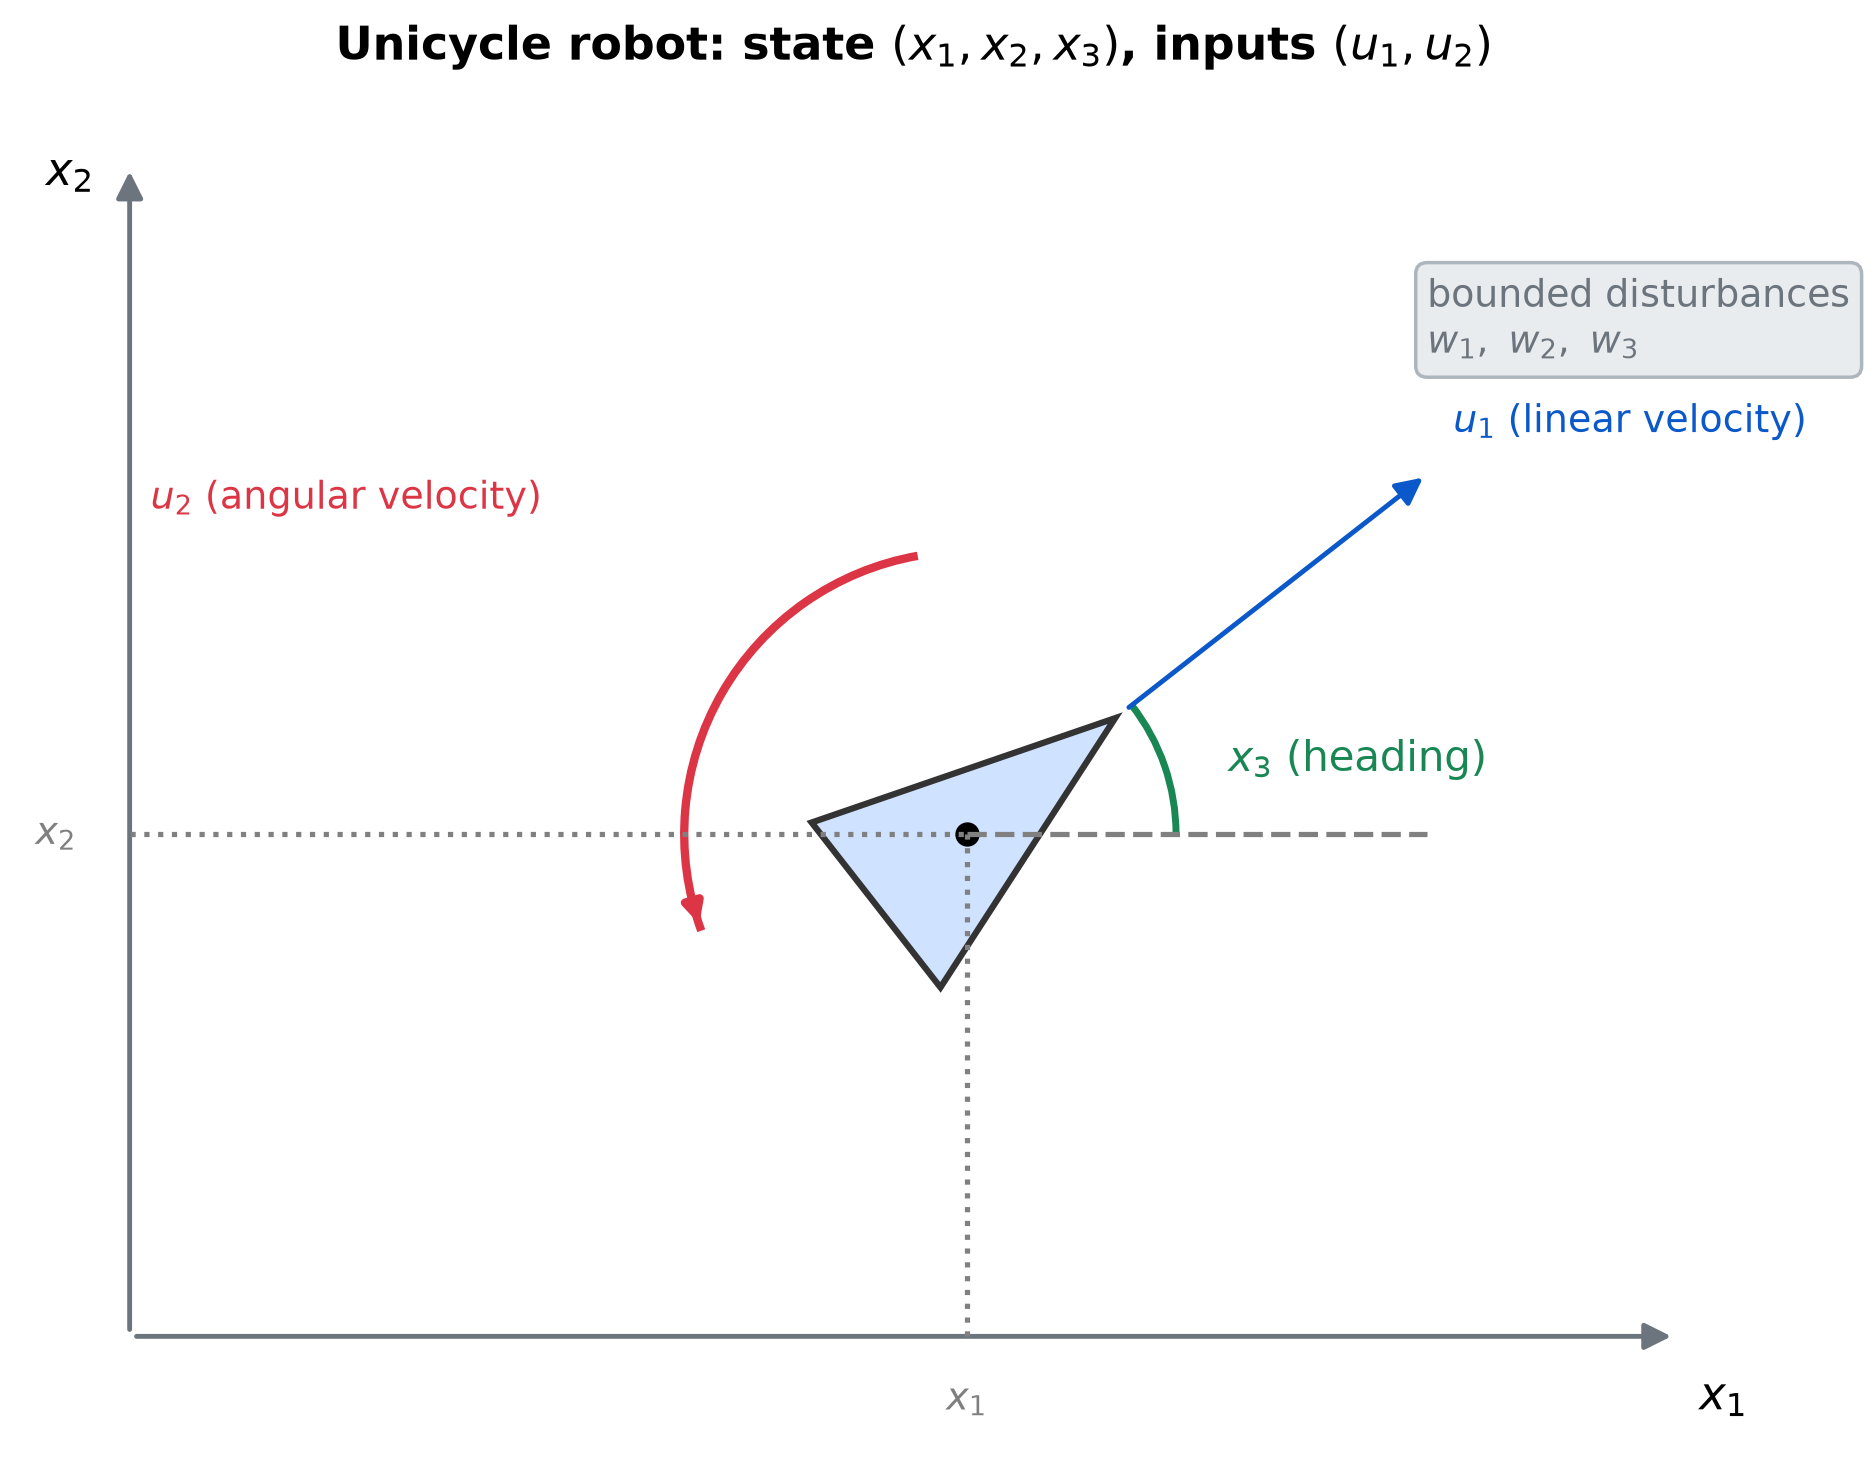
\includegraphics[width=.82\linewidth,height=.43\textheight,keepaspectratio]{robot_model.png}
 \caption{The robot state variables and control inputs.}
\end{figure}

The workspace is $X=[0,10]\times[0,10]\times[-\pi,\pi]$.
We keep $\tau$, the command bounds and disturbance half-widths symbolic in the derivation below.

\begin{table}[!htbp]
 \centering
 \caption{Regions defined in the reference article. The heading is unrestricted in every region.}
 \renewcommand{\arraystretch}{1.2}
 \begin{tabular}{lll}
 \toprule
 Region & Position domain $(x_1(t),x_2(t))$ & Role\\
 \midrule
 $R_1$ & $[4,5]\times[8.5,9.5]$ & First destination, option 1\\
 $R_2$ & $[8.5,9.5]\times[2,3]$ & First destination, option 2\\
 $R_3$ & $[2,3]\times[0.5,1.5]$ & Subsequent destination\\
 $R_4$ & $[3,7]\times[3,7]$ & Obstacle to avoid\\
 \bottomrule
 \end{tabular}
\end{table}

We read the specification as choosing exactly one of $R_1$ and $R_2$,
then reaching $R_3$, while avoiding $R_4$ throughout the task.
This helped us see why the current position alone does not record progress:
we also need to remember which first destination has been visited.

\begin{figure}[H]
 \centering
 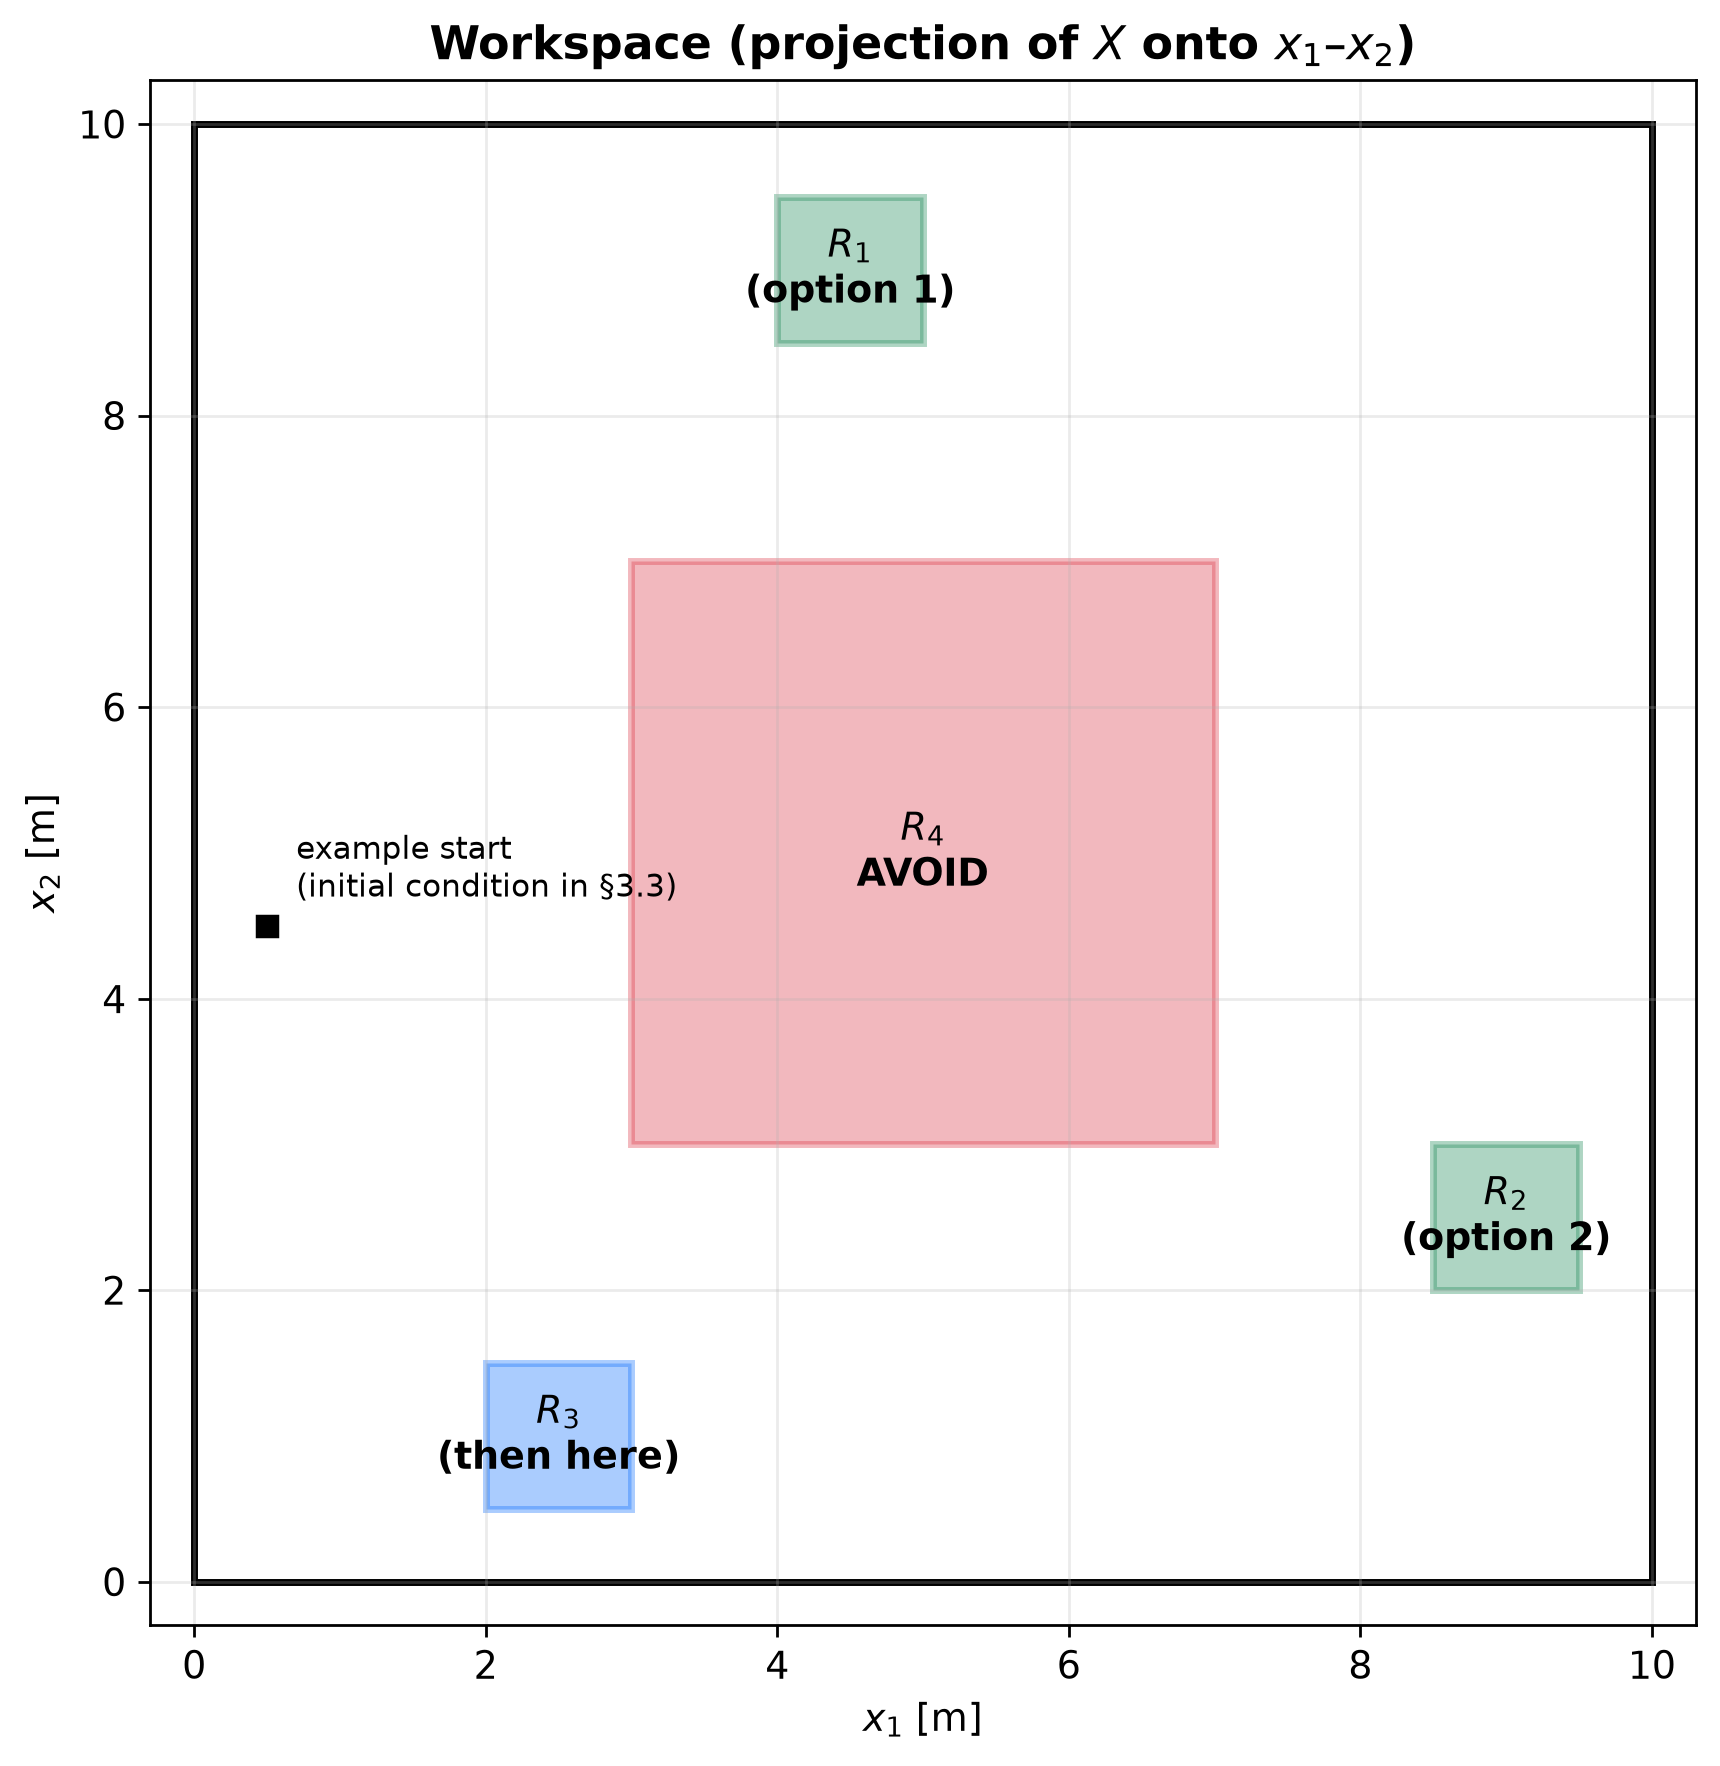
\includegraphics[width=.68\linewidth,height=.43\textheight,keepaspectratio]{robot_workspace.png}
 \caption{The four regions in the position plane. The marked starting point
 is illustrative; no closed-loop trajectory has been implemented by our group.}
\end{figure}

This memory is represented by a five-state automaton: state
$0$ means no first destination has been visited; states $1$ and $2$ record
visiting $R_1$ or $R_2$; state $3$ records completion; state $4$ records
failure. Entering the obstacle or visiting the other first destination
before completion leads to failure. In this co-safe interpretation,
completion and failure are absorbing states: the automaton evaluates the
finite task up to completion, rather than imposing an additional perpetual
safety requirement afterwards.

\begin{figure}[H]
 \centering
 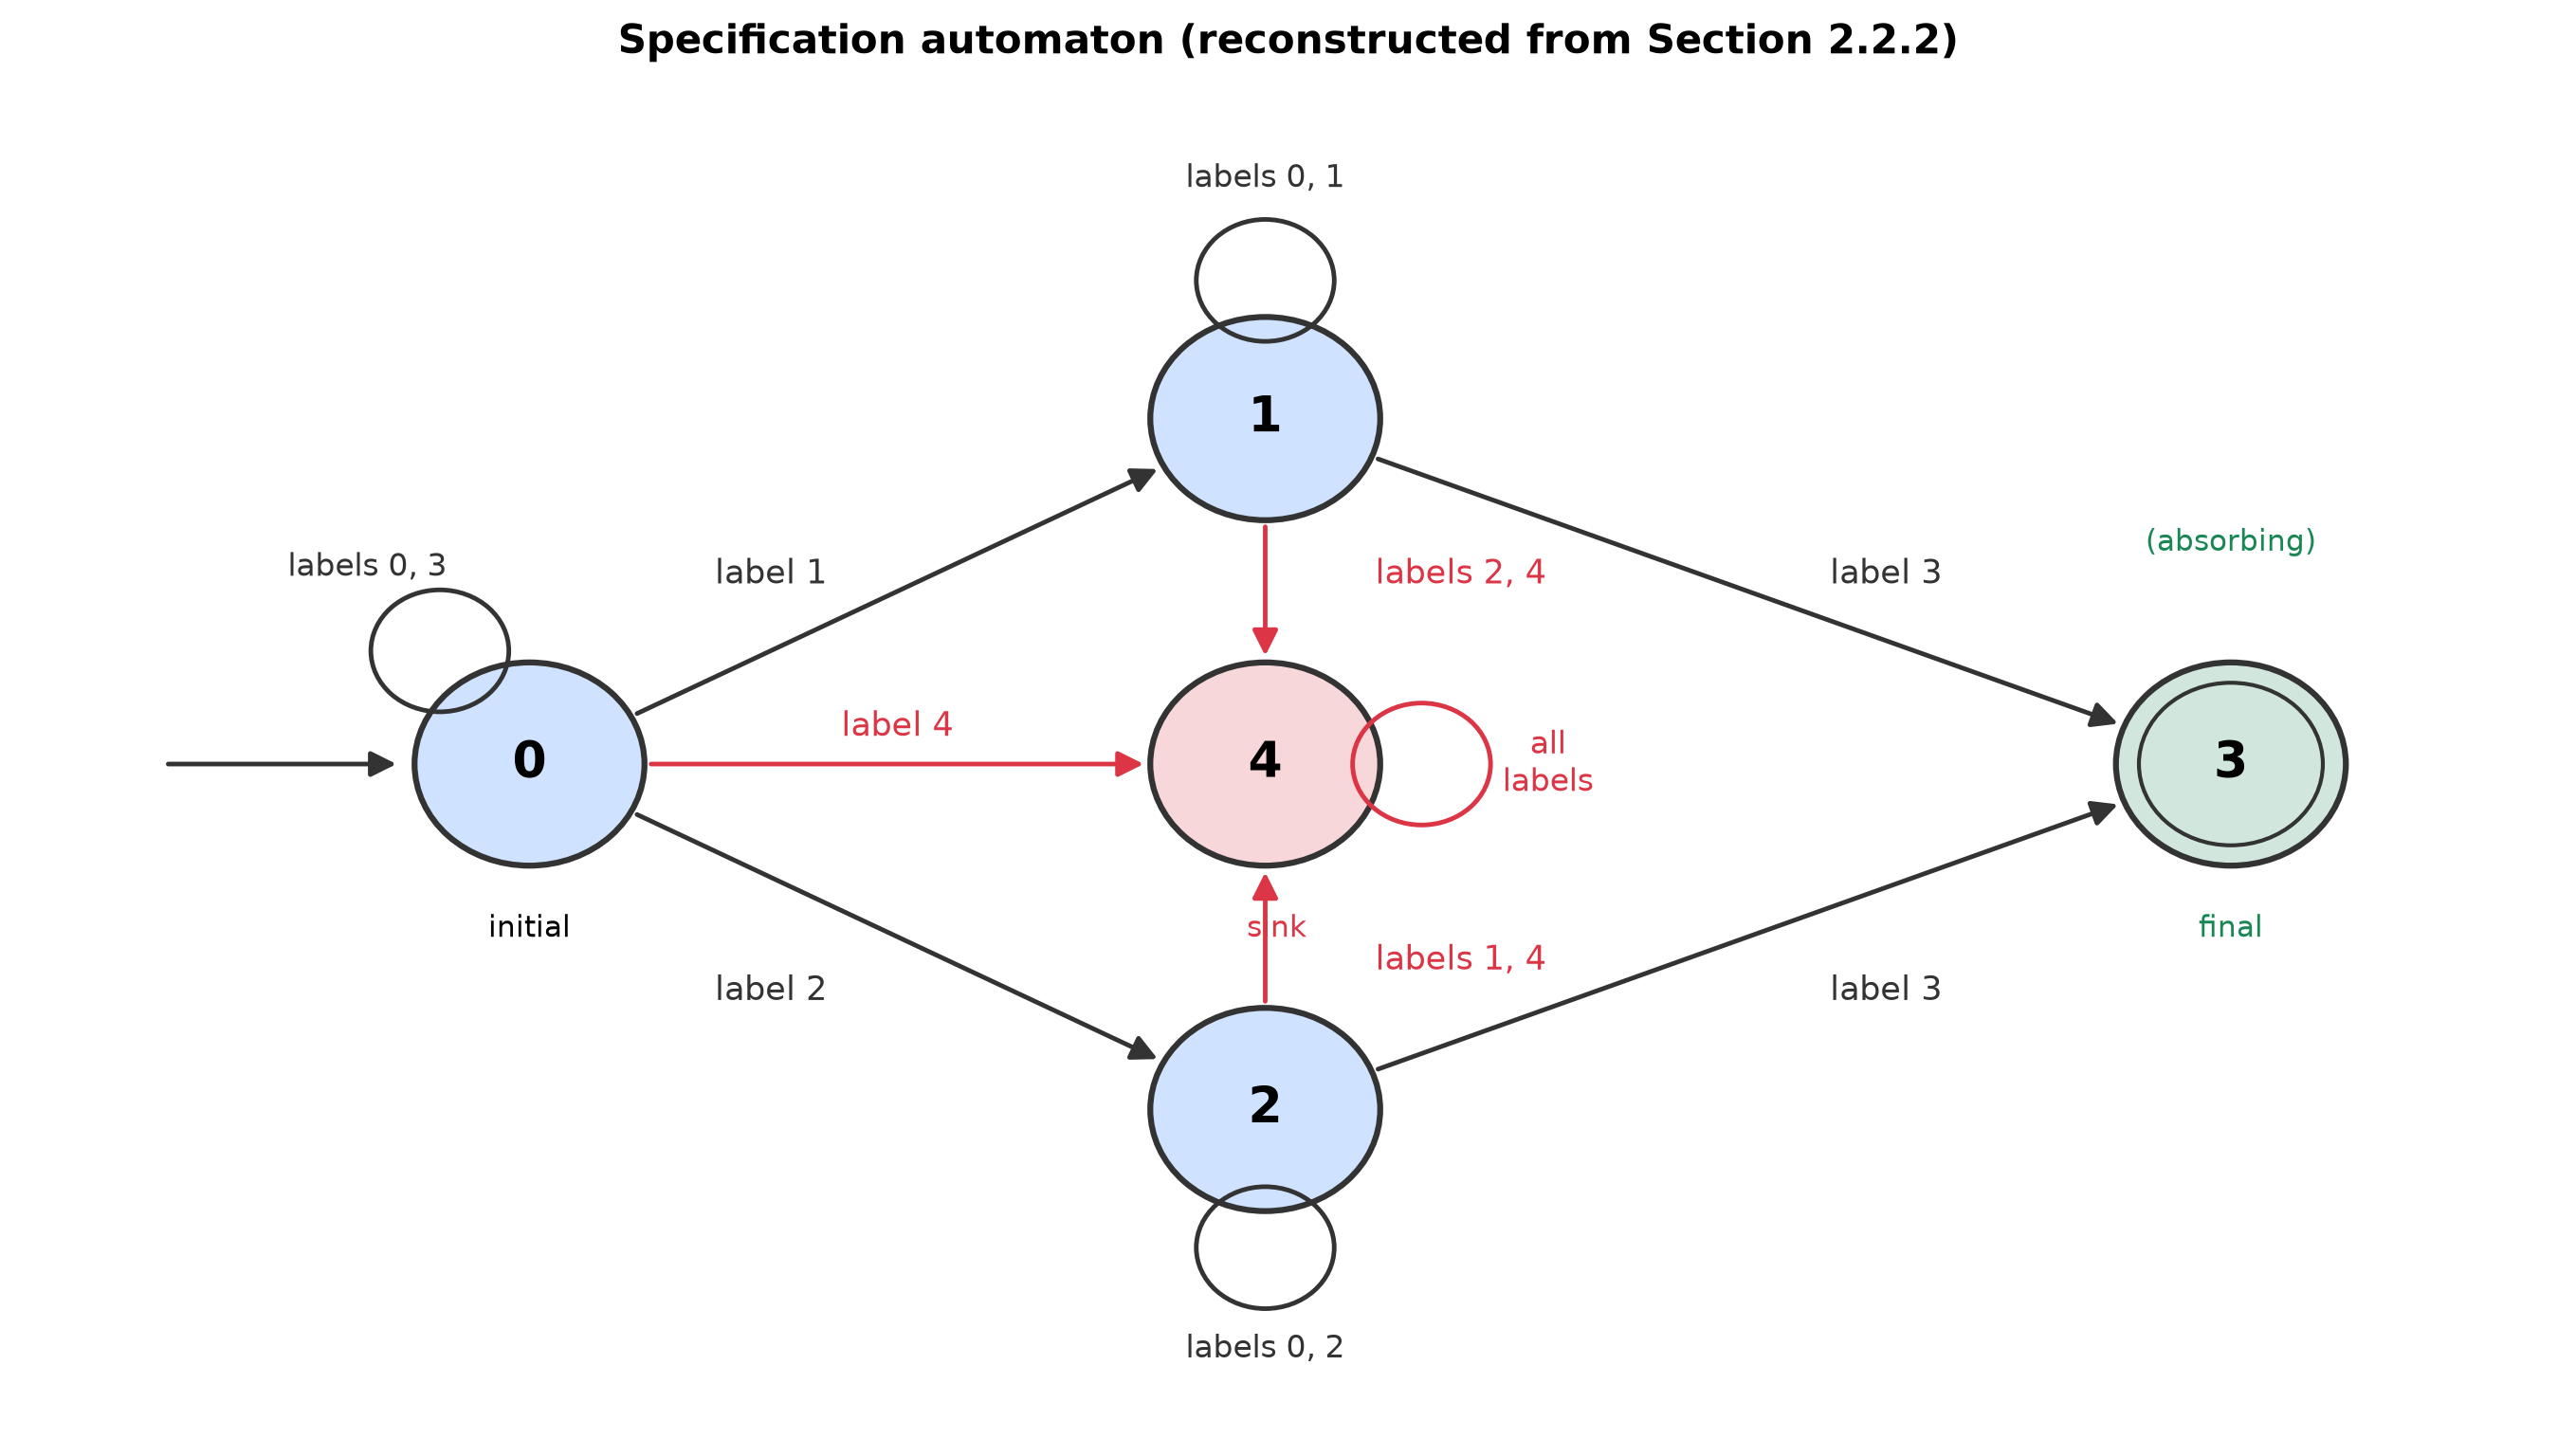
\includegraphics[width=\linewidth,height=.43\textheight,keepaspectratio]{specification_automaton.png}
 \caption{The specification automaton. Label $i$
 denotes region $R_i$; label $0$ denotes a point outside all four regions.}
\end{figure}

\FloatBarrier
\FloatBarrier
\subsubsection{Robot discretization: the beginning of Section 3.2}
We followed the same abstraction steps with a uniform Cartesian partition:
\[
 N_1=100,\qquad N_2=100,\qquad N_3=30.
\]
This gives $100\times100\times30=300\,000$ cells and
$300\,001$ symbolic states when the outside state is included. Each cell
has full widths
\[
 h=\left(0.1\ \mathrm m,\;0.1\ \mathrm m,\;
 \frac{2\pi}{30}\ \mathrm{rad}\right),\qquad \delta x=\frac h2.
\]
The selected input set combines three linear-velocity values and five
angular-velocity values, giving $3\times5=15$ symbolic commands.
These are the discretization sizes discussed in the article; they are
not results of an implementation completed by our group.

\FloatBarrier
\subsubsection{Derivative bounds and the size of the enclosure}
The robot is not globally monotone in the standard componentwise order:
\[
 \frac{\partial f_1}{\partial x_3(t)}=-\tau u_1(t)\sin x_3(t)
\]
changes sign with the heading. We therefore understood why the bounded
derivative method is used. Differentiating the robot model gives
\[
 \frac{\partial f}{\partial x(t)}=
 \begin{pmatrix}
 1&0&-\tau u_1(t)\sin x_3(t)\\
 0&1&\tau u_1(t)\cos x_3(t)\\
 0&0&1
 \end{pmatrix},\qquad
 \frac{\partial f}{\partial w(t)}=\tau I_3.
\]
With $|u_1|_{\max}=\max_{u\in U}|u_1|$, and using
$|\sin x_3(t)|\le1$, $|\cos x_3(t)|\le1$, uniform bounds are
\[
 D_x=\begin{pmatrix}
 1&0&\tau|u_1|_{\max}\\
 0&1&\tau|u_1|_{\max}\\
 0&0&1
 \end{pmatrix},\qquad D_w=\tau I_3.
\]
Thus $G(\xi,\sigma)=[f(x^*(t),u_\sigma,w^*)-r,
f(x^*(t),u_\sigma,w^*)+r]$. Because the grid is uniform and the same global
derivative bounds are used for every cell and command, its half-widths
are constant. Its centre changes with the cell and command; its size
does not. This is the point at which we stopped during our first meeting:

\begin{tcolorbox}[title={Consequence: the same enclosure size for every cell}]
\begin{equation}
 \boxed{\begin{aligned}
 r_1&=\delta x_1+\tau|u_1|_{\max}\,\delta x_3+\tau\,\delta w_1,\\
 r_2&=\delta x_2+\tau|u_1|_{\max}\,\delta x_3+\tau\,\delta w_2,\\
 r_3&=\delta x_3+\tau\,\delta w_3.
 \end{aligned}}
\end{equation}
\end{tcolorbox}

\FloatBarrier


\subsection{Implementation}
% To be completed (step 2): code, results, computation time.
\begin{tcolorbox}[title={Second meeting --- 11 October 2026}]
During our second meeting we figured that not only did we need to master the theory,
but also bring it to life via implementation. Down below is the overview of the work completed during that point.
\end{tcolorbox}

% Helper (local to this part): keep a listing caption with the start of its code.
\providecommand{\needroom}[1]{\par\begingroup\dimen0=\pagegoal\advance\dimen0 by -\pagetotal\ifdim\dimen0<#1 \newpage\fi\endgroup}
\subsubsection{Overview of the implementation}
For the implementation of the symbolic abstraction, we need to divide our attention into three
sub-problems. Two of them are conversion mechanisms: the conversion from the state
coordinates to the state ID, and the inverse conversion from the state ID back to the actual
state coordinates. Last but not least, we tackle the implementation of the dynamics, which, as
an overview, covers the essential mathematical basis (Jacobians, bounds of each continuous
input, etc.). Once these three subtasks are completed, we move on to the assembly. In other
words, we use them to construct the whole logic behind the symbolic abstraction of our problem.

\subsubsection{Subtask 1: \texttt{coord2state.hpp}}
Let us start with the first subtask, namely the first \texttt{.hpp} file in our
\texttt{symbolicAbstraction} folder, \texttt{coord2state}:

\needroom{9\baselineskip}
\begin{lstlisting}[language=C++,caption={\texttt{coord2state.hpp}: from cell coordinates to a unique state ID.}]
// C++ port of coord2state.m
// Grid coordinates (one index per dimension, 1-based) -> single state number (1-based).
// MATLAB: i = (I-1)' * p_x(1:length(I)) + 1
#pragma once
#include <array>

template <size_t N>
int coord2state(const std::array<int, N>& I, const std::array<int, N + 1>& p) {
    int i = 1;
    for (size_t k = 0; k < N; ++k) i += (I[k] - 1) * p[k];
    return i;
}
\end{lstlisting}

\paragraph{Explanation/Analysis.}
This file only needs one function. It takes as a parameter an input array of coordinates, which
are cell numbers, each coming from the continuous input parameters. For instance, if our robot
is at $(x_1,x_2,x_3)$, we ask: what does this translate to in our discrete representation? To do
that, $x_1$ is mapped to a certain interval, as discussed in the discretization process, which
gives us a certain cell, and the same goes for the other coordinates. So the goal here is to get
those cell coordinates, together with a hash-like array which allows us to yield a unique ID for
the exact cell our robot inhabits at the real coordinates $(x_1,x_2,x_3)$.

The hash-like array is none other than $(1,\,100,\,10\,000,\,300\,000)$, but why? After the
discretization, the $x_1$ values fit into 100 bins (intervals), the same holds for $x_2$, and
there are 30 bins for $x_3$, so the mapping array is of the form
$(1,\,n_{x_1},\,n_{x_1}n_{x_2},\,n_{x_1}n_{x_2}n_{x_3})$. We can read the numerical values as
follows: if only $x_1$ changes, we move to the neighbouring cell (a step of 1). If we hold $x_1$
fixed and move along $x_2$, we move by 100 cells in the matrix. However, if we fix $x_1$ and
$x_2$ and vary $x_3$, we move by blocks of $100\times100$ ($x_1\times x_2$). Using this logic, we
get the exact ID of the cell in the discrete grid of $300\,000$ cells built in the theory above.

\subsubsection{Subtask 2: \texttt{state2coord.hpp}}
Now moving on to the second concern. Given a state ID (a cell) among the $300\,000$ discrete
states, how can we know from which bins it was yielded? The answer lies inside our second
\texttt{.hpp} file, \texttt{state2coord}:

\needroom{9\baselineskip}
\begin{lstlisting}[language=C++,caption={\texttt{state2coord.hpp}: from a state ID back to cell coordinates.}]
// C++ port of state2coord.m
// Single state number (1-based) -> grid coordinates (one index per dimension, 1-based).
// MATLAB: I(k) = floor(mod(i-1, p(k+1)) / p(k)) + 1
#pragma once
#include <array>

template <size_t N>
std::array<int, N> state2coord(int i, const std::array<int, N + 1>& p) {
    std::array<int, N> I;
    for (size_t k = 0; k < N; ++k) I[k] = ((i - 1) % p[k + 1]) / p[k] + 1;
    return I;
}
\end{lstlisting}

\paragraph{Explanation/Analysis.}
This file also needs only one function. It takes as parameters the state ID and, of course, the
hash-like array, in order to backtrack all the way to the origin, meaning the cell coordinates
and not the real $(x_1,x_2,x_3)$, because the mapping is not bijective in that sense. Using that
formula, we return the wanted result.

\begin{tcolorbox}[title={Note}]
This function is used mainly when dealing with the concretization of the action input $u$, where
we get a discrete input (from 1 to 15, since we have 3 discrete values for the linear velocity
and 5 discrete values for the angular velocity). This is discussed below; let us save it for later.
\end{tcolorbox}

\subsubsection{Subtask 3: \texttt{dynamics.hpp}}
The last, but not least, \texttt{.hpp} file is \texttt{dynamics}. In this file we set our dynamics
function $f$, that of the real movement of the robot, the Jacobian matrices modelling the
derivatives with respect to each of the function's parameters, as well as the several bounds and
discretization settings:

\needroom{9\baselineskip}
\begin{lstlisting}[language=C++,caption={\texttt{dynamics.hpp}: dynamics, Jacobian bounds, constraints and discretization settings.}]
// C++ port of dynamics.m
// Defines the system (unicycle), its bounds, and the abstraction grid sizes.
#pragma once
#include <array>
#include <cmath>

using Vec3 = std::array<double, 3>;
using Vec2 = std::array<double, 2>;
using Mat3 = std::array<std::array<double, 3>, 3>;
using Idx3 = std::array<int, 3>;
using Idx2 = std::array<int, 2>;

constexpr double PI = 3.14159265358979323846;

namespace dyn {

// Sampling time
constexpr double T = 1.0;

// System dynamics  x+ = f(x,u,w)
inline Vec3 f(const Vec3& x, const Vec2& u, const Vec3& w) {
    return {x[0] + T * u[0] * std::cos(x[2]) + T * w[0],
            x[1] + T * u[0] * std::sin(x[2]) + T * w[1],
            x[2] + T * u[1] + T * w[2]};
}

// Bounds on the Jacobian matrices (used to over-approximate reachable sets)
inline Mat3 Jf_x(const Vec2& u) {
    const double a = T * std::fabs(u[0]);
    return {{{1, 0, a},
             {0, 1, a},
             {0, 0, 1}}};
}

inline Mat3 Jf_w(const Vec2& /*u*/) {
    return {{{T, 0, 0},
             {0, T, 0},
             {0, 0, T}}};
}

// Constraints: first = lower bound, second = upper bound
constexpr Vec3 bound_x_lo = {0.0, 0.0, -PI};
constexpr Vec3 bound_x_hi = {10.0, 10.0, PI};
constexpr Vec2 bound_u_lo = {0.25, -1.0};
constexpr Vec2 bound_u_hi = {1.0, 1.0};
constexpr Vec3 bound_w_lo = {-0.05, -0.05, -0.05};
constexpr Vec3 bound_w_hi = {0.05, 0.05, 0.05};

// Abstraction parameters: number of cells per dimension
constexpr Idx3 n_x = {100, 100, 30};
constexpr Idx2 n_u = {3, 5};

}  // namespace dyn
\end{lstlisting}

\paragraph{Explanation/Analysis.}
\begin{itemize}
  \item \textbf{The robot function model.} As modelled mathematically, the function takes three
  parameters: a positional one, an actionable one, and a last one dedicated to the disturbances
  that might occur in each of the positional parameters due to sensor precision, etc. The
  function returns a vector containing the three equations modelling the robot's movements on
  the plane.
  \item \textbf{The Jacobian matrices.} This one is pretty self-explanatory: the derivative with
  respect to $x$ depends on $u$ and the constant $T$, whereas the derivative with respect to $w$
  only depends on the constant $T$. This is mathematically sound and clear.
  \item \textbf{The bounds.} Of course, they are given by the problem setting and are very
  essential for the dynamics of the robot (pretty self-explanatory too).
  \item \textbf{The discretization setting.} As stated in the theory part of this
  implementation, we opted for a $\{100,100,30\}$ discretization for $x_1,x_2,x_3$ respectively,
  yielding $300\,000$ cells/states. As for $u$, the discrete setting is $\{3,5\}$, yielding 15
  control actions.
\end{itemize}

The implementation of these subtasks truly simplifies the coding aspect of the core symbolic
abstraction. We will see how and why in our next segment, in which we discuss the process that
leads us to it.

\subsubsection{Assembly: \texttt{symb\_abs.cpp}}
Our next file is \texttt{symb\_abs}, which is the first \texttt{.cpp} file.

\paragraph{Helper method.}
First of all, we defined a helper method to bypass any matrix--vector multiplication.

\needroom{9\baselineskip}
\begin{lstlisting}[language=C++,caption={Matrix--vector multiplication helper.}]
static Vec3 matvec(const Mat3& M, const Vec3& v) {
    Vec3 r{};
    for (int i = 0; i < 3; ++i)
        for (int j = 0; j < 3; ++j) r[i] += M[i][j] * v[j];
    return r;
}
\end{lstlisting}

\textbf{Explanation/Analysis.} This helper needs no further explanation.

\paragraph{State discretization.}
Second is the state discretization. We discretize each of our positional parameters
$(x_1,x_2,x_3)$ like so:

\needroom{9\baselineskip}
\begin{lstlisting}[language=C++,caption={State discretization.}]
Vec3 d_x;
for (int i = 0; i < 3; ++i) d_x[i] = (bound_x_hi[i] - bound_x_lo[i]) / n_x[i];
const std::array<int, 4> p_x = {1, n_x[0], n_x[0] * n_x[1], n_x[0] * n_x[1] * n_x[2]};
const int n_xi = p_x[3];
\end{lstlisting}

\textbf{Explanation/Analysis.}
\begin{itemize}
  \item We have, for both $x_1$ and $x_2$, as we saw, a width of $0.1$ for each state, and for
  $x_3$ it is $\frac{2\pi}{30}$, in conformity with the theory discussed above.
  \item We also build our hash-like array \texttt{p\_x} in the same way as discussed before.
  \item We set the number of all possible states resulting from our discretization from
  \texttt{p\_x[3]}, which, as discussed, is the correct thing to do.
\end{itemize}

\paragraph{Input discretization.}
Third is the input discretization. We discretize the linear velocity as well as the angular
velocity just like so:

\needroom{9\baselineskip}
\begin{lstlisting}[language=C++,caption={Input discretization.}]
Vec2 d_u;
for (int i = 0; i < 2; ++i) d_u[i] = (bound_u_hi[i] - bound_u_lo[i]) / (n_u[i] - 1);
const std::array<int, 3> p_u = {1, n_u[0], n_u[0] * n_u[1]};
const int n_sigma = p_u[2];
\end{lstlisting}

\textbf{Explanation/Analysis.}
\begin{itemize}
  \item Here it is good to note that we divide by \texttt{n\_u[i] - 1}, to avoid the cardinality
  mistake coming from redundant values in two consecutive bins.
  \item Same as for the state, except that here we build \texttt{p\_u}, which contains at its
  third slot \texttt{p\_u[2]} the number of discrete inputs \texttt{n\_sigma}.
\end{itemize}

\paragraph{Concretization function.}
Fourth is the concretization function. As we discussed in the theory, for the actions
$(u_1,u_2)$ we need a concretization function, since our robot does not understand the discretized
values $(1,\dots,15)$; it understands velocities. Here, we make use of our \texttt{state2coord}
function and apply a transformation to know the actual yielder of each of the states.

\needroom{9\baselineskip}
\begin{lstlisting}[language=C++,caption={Concretization function.}]
std::vector<Vec2> val_u(n_sigma);
for (int i = 1; i <= n_sigma; ++i) {
    Idx2 c = state2coord<2>(i, p_u);
    for (int k = 0; k < 2; ++k) val_u[i - 1][k] = bound_u_lo[k] + (c[k] - 1) * d_u[k];
}
\end{lstlisting}

\textbf{Explanation/Analysis.}
\begin{itemize}
  \item As you can clearly see, we use all the possible discrete inputs, which are between 1
  and 15 according to the problem specifications. Now the goal is to know what yielded each of
  them. So we build a $15\times2$ matrix, such that row $i$ is the yielder of the state $i+1$.
  \item The mathematical transformation is clear, and we confirmed that it works.
\end{itemize}

\paragraph{Disturbance setup.}
Fifth is the disturbance setup to start the symbolic abstraction, and it goes like this:

\needroom{9\baselineskip}
\begin{lstlisting}[language=C++,caption={Disturbance setup.}]
Vec3 d_w, w_c;
for (int i = 0; i < 3; ++i) {
    d_w[i] = bound_w_hi[i] - bound_w_lo[i];
    w_c[i] = 0.5 * (bound_w_lo[i] + bound_w_hi[i]);
}
\end{lstlisting}

\textbf{Explanation/Analysis.}
\begin{itemize}
  \item We compute both \texttt{d\_w} and the center \texttt{w\_c}, since both are essential for
  the computation of the reachable set.
\end{itemize}

\paragraph{Simulation: computation of the reachable set.}

\needroom{9\baselineskip}
\begin{lstlisting}[language=C++,caption={Over-approximation of the reachable set.}]
Vec3 x_c_succ = f(x_c, u, w_c);
Vec3 a = matvec(Jf_x(u), d_x);
Vec3 b = matvec(Jf_w(u), d_w);
Vec3 reach_lo, reach_hi;
for (int i = 0; i < 3; ++i) {
    double dev = 0.5 * a[i] + 0.5 * b[i];
    reach_lo[i] = x_c_succ[i] - dev;
    reach_hi[i] = x_c_succ[i] + dev;
}
\end{lstlisting}

\textbf{Explanation/Analysis.}
In the simulation we discuss a very important aspect of this symbolic abstraction. Without it, we
would not be able to establish reachability, which is a pillar of our project. In a similar
fashion to what we discussed in the theory, we need to multiply the Jacobians by their respective
maximal step (the amplitude/length of the intervals). We apply this to the movement
$(x_1,x_2,x_3)$ and we also take the disturbance into account. This yields two bounds, a low and a
high one, which determine the whole reachable set. Of course, this set might not represent
\emph{one} exact cell in our discretized grid. In this case, which is the most likely to happen
each time, we take the intersection of our grid cells with that reachable set. This implies that
our robot, in the discretized setting, can reach all of those cells.

\needroom{9\baselineskip}
\begin{lstlisting}[language=C++,caption={Cells intersected by the reachable set.}]
Idx3 cmin, cmax;
for (int i = 0; i < 3; ++i) {
    cmin[i] = (int)std::floor((reach_lo[i] - bound_x_lo[i]) / d_x[i]) + 1;
    cmax[i] = (int)std::ceil((reach_hi[i] - bound_x_lo[i]) / d_x[i]);
}
g[(size_t)(xi - 1) * n_sigma + (sigma - 1)] = {coord2state<3>(cmin, p_x),
                                               coord2state<3>(cmax, p_x)};
\end{lstlisting}

\begin{tcolorbox}[title={Goal}]
With this process we build the transition function, which makes complete sense: from each cell,
given an action, we compute the reachable states/cells. It is the same as
\[
 \sigma(q,a)\;\longrightarrow\;\{\,q_i \mid q_i\in\text{Reachable set}\,\}.
\]
\end{tcolorbox}

% ============================================================
\section{Symbolic Controller Synthesis}
\label{sec:synthesis}
% ============================================================

\subsection{Theory}
% To be completed (step 3): automaton product, reachability synthesis.

\subsection{Implementation}
% To be completed (step 3): code, number of iterations, computation time.

% ============================================================
\section{Concretization and Simulation}
\label{sec:concretization}
% ============================================================

% To be completed (step 4): concretized controller, closed-loop trajectories.

% ============================================================
\section{Conclusion}
% ============================================================

% To be completed.

% Add future project parts here with \part{...}.
\end{document}